\documentclass{article}
\usepackage{caption}
\usepackage{amsmath, fullpage}
\usepackage{tikz}
\usepackage{booktabs}
\usetikzlibrary{calc,arrows.meta}


\begin{document}

\title{Data Structures \& Algorithms}
\author{Edward Song}
\maketitle
\thispagestyle{empty}

\section{Arrays}

\subsection{Definition}
An \textbf{array} is a data structure that stores elements in \textbf{contiguous blocks of memory}.  
Each element can be accessed directly using its index.

\subsection{Memory Layout}
\begin{figure}[h]
\centering
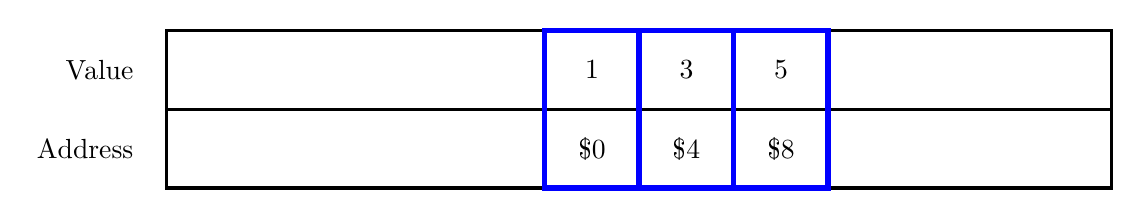
\begin{tikzpicture}[x=1cm,y=1cm]

% --- Geometry settings ---
\def\W{12}        % total width of the big memory block
\def\H{2}         % total height (2 rows)
\def\cellW{1.2}   % width of each cell in the highlighted region
\def\nCells{3}
\def\hiX{4.8}     % x-position where the highlighted region starts (centered-ish)

% --- Outer "RAM block" rectangle and the row divider ---
\draw[line width=1.2pt] (0,0) rectangle (\W,\H);
\draw[line width=1.2pt] (0,1) -- (\W,1);

% --- Labels on the left (no overlap) ---
\node[anchor=east] at (-0.3,1.5) {Value};
\node[anchor=east] at (-0.3,0.5) {Address};

% --- Highlighted region: contiguous cells spanning both rows ---
% Outer highlight frame
\draw[draw=blue, line width=2pt] (\hiX,0) rectangle ({\hiX+\nCells*\cellW},\H);

% Internal vertical dividers for each cell
\foreach \i in {1,...,2} {
  \draw[draw=blue, line width=2pt]
    ({\hiX+\i*\cellW},0) -- ({\hiX+\i*\cellW},\H);
}

% --- Text inside cells ---
\node at ({\hiX+0.5*\cellW},1.5) {1};
\node at ({\hiX+1.5*\cellW},1.5) {3};
\node at ({\hiX+2.5*\cellW},1.5) {5};

\node at ({\hiX+0.5*\cellW},0.5) {\$0};
\node at ({\hiX+1.5*\cellW},0.5) {\$4};
\node at ({\hiX+2.5*\cellW},0.5) {\$8};

\end{tikzpicture}
\caption{Arrays are stored in contiguous blocks of memory}
\end{figure}


Because memory is contiguous, the address of any element can be computed in constant time:
\[
\text{address}(i) = \text{base} + i \cdot \text{sizeof(element)}
\]

\subsection{Types of Arrays}

\textbf{Static Arrays}
\begin{itemize}
  \item Fixed size determined at creation time
  \item Stored in one continuous block of memory
  \item Cannot grow or shrink
  \item Memory-efficient (no resizing overhead)
\end{itemize}
\textbf{Dynamic Arrays}
\begin{itemize}
  \item Automatically resize when capacity is reached
  \item Implemented using an underlying static array
  \item When full:
    \begin{itemize}
      \item A new array (usually 2× larger) is allocated
      \item All elements are copied to the new array
      \item Old array is deallocated
    \end{itemize}
  \item Appending is \textbf{amortized} to $O(1)$
\end{itemize}

\subsection{Time Complexity}

\begin{center}
\begin{tabular}{l c}
\toprule
\textbf{Operation} & \textbf{Time Complexity} \\
\midrule
Read by index & $O(1)$ \\
Write at end (append) & $O(1)$ \\
Insert at beginning & $O(n)$ \\
Insert in middle & $O(n)$ \\
Insert at end & $O(1)$ \\
Remove from beginning & $O(n)$ \\
Remove from middle & $O(n)$ \\
Remove at end & $O(1)$ \\
\bottomrule
\end{tabular}
\end{center}

\subsection{Why Some Operations Are Slow}
Inserting or removing elements at the beginning or middle of an array requires shifting all subsequent elements to preserve contiguous memory, which is $O(n)$.
\input{sections/02-stacks}
\section{Linked Lists}

A \textbf{singly linked list} is a linear data structure made of \textbf{nodes}.  
Each node stores:
\begin{itemize}
  \item a value (data)
  \item a pointer/reference to the next node
\end{itemize}

The last node points to \texttt{null}.

\begin{figure}[h]
\centering
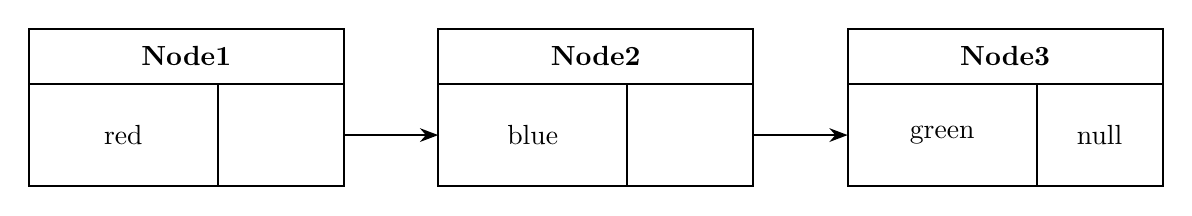
\begin{tikzpicture}[
  >=Stealth,
  pointer/.style={->, thick}
]

% --- Node drawing helper: (x,y), title, value, next ---
\newcommand{\ListNode}[5]{%
  % Outer box
  \draw[thick] (#1,#2) rectangle ++(4,2);

  % Header divider
  \draw[thick] (#1,#2+1.3) -- ++(4,0);

  % Body vertical divider (value | next)
  \draw[thick] (#1+2.4,#2) -- ++(0,1.3);

  % Header text
  \node at (#1+2,#2+1.65) {\textbf{#3}};

  % Value / Next text
  \node at (#1+1.2,#2+0.65) {#4};
  \node at (#1+3.2,#2+0.65) {#5};
}

% --- Draw nodes ---
\ListNode{0}{0}{Node1}{red}{}
\ListNode{5.2}{0}{Node2}{blue}{}
\ListNode{10.4}{0}{Node3}{green}{null}

% --- Straight arrows (from next-field center to next node) ---
\draw[pointer] (4,0.65) -- (5.2,0.65);
\draw[pointer] (9.2,0.65) -- (10.4,0.65);

\end{tikzpicture}
\caption{A singly linked list where each node points to the next node}
\end{figure}



\subsection{Memory Layout}
Unlike arrays, linked lists are \textbf{not stored contiguously in memory}.  
Nodes can be located anywhere in memory and are connected using pointers.

\subsection{Structure}
\begin{itemize}
  \item \textbf{Head}: first node in the list
  \item \textbf{Tail}: last node in the list (points to \texttt{null})
\end{itemize}


\subsection{Traversal}
To iterate through a linked list:
\begin{verbatim}
curr = head
while (curr != null):
    curr = curr.next
\end{verbatim}
Traversal takes $O(n)$ time, where $n$ is the number of nodes.

\subsection{Insertion and Deletion}

\textbf{Inserting a node (given previous node)}
\begin{verbatim}
    newNode.next = prev.next
    prev.next = newNode
\end{verbatim}
\textbf{Deleting a node (given previous node):}
\begin{verbatim}
    prev.next = prev.next.next
\end{verbatim}
\textbf{Inserting before the head:}
\begin{verbatim}
    newNode.next = head
    head = newNode
\end{verbatim}
\textbf{Deleting the head:}
\begin{verbatim}
    head = head.next
\end{verbatim}

Inserting or deleting a node itself is $O(1)$, but finding the previous node takes $O(n)$ due to the lack of random access, so the overall operation is $O(n)$ if a search is required.

\subsection{Time Complexity}

\begin{center}
\begin{tabular}{l c}
\toprule
\textbf{Operation} & \textbf{Time Complexity} \\
\midrule
Access by index & $O(n)$ \\
Insert at head & $O(1)$ \\
Insert at tail & $O(1)$ (with tail pointer) \\
Insert in middle & $O(n)$ \\
Delete at head & $O(1)$ \\
Delete at tail & $O(n)$ \\
Delete in middle & $O(n)$ \\
\bottomrule
\end{tabular}
\end{center}

\subsection{Doubly Linked Lists}
In a \textbf{doubly linked list}, each node stores two pointers:
\begin{itemize}
  \item \texttt{next}: points to the next node
  \item \texttt{prev}: points to the previous node
\end{itemize}

This allows traversals forwards or backwards and enables insertions and deletions to be performed without needing to find the previous node, resulting in $O(1)$ when deleting at the end. Insertions/Deletions in the middle of the list are still $O(n)$, as we still need to access the i-th element.
\section{Queues}

A \textbf{queue} is a data structure that supports insertion at one end and removal at the other.  
The simplest way a queue be implemented is using a \textbf{linked list} with head and tail pointers.

\subsection{Core Operations}
\begin{itemize}
  \item \textbf{Enqueue:} add an element to the back of the queue (tail)
  \item \textbf{Dequeue:} remove an element from the front of the queue (head)
\end{itemize}
Enqueue and Dequeue are both \textbf{$O(1)$} since we maintain pointers to the head and tail.

\subsection{Ordering Property}
Queues are \textbf{FIFO} (\textit{First In, First Out}):
\[
\text{Enqueue: } 1,2,3 \quad \Rightarrow \quad \text{Dequeue: } 1,2,3
\]
\section{Recursion}

\textbf{Recursion} is a programming technique where a function calls itself to solve a problem by breaking it into smaller subproblems.  
Every recursive function must have a \textbf{base case} to stop the recursion.

\subsection{Memory Model}
Each function call (recursive or not) creates a new \textbf{stack frame} on the call stack, which stores:
\begin{itemize}
  \item local variables
  \item parameters
  \item return address
\end{itemize}
Recursive calls create multiple stack frames, which are removed as the function returns. Recursive depth determines stack memory usage.

\subsection{Example: Factorial}

Computing factorials with a for loop:
\begin{verbatim}
int factorial(int n) {
    int result = 1;
    for (int i = 1; i <= n; i++) {
        result *= i;
    }
    return result;
}
\end{verbatim}
Computing factorials with recursion:
\begin{verbatim}
int factorial(int n) {
    if (n <= 1) {
        return 1;   // base case
    }
    return n * factorial(n - 1);
}
\end{verbatim}

\subsection{Example: Fibonacci}
Computing fibonacci with recursion:
\begin{verbatim}
int fib(int x) {
    if (x == 1) {
        return 1;
    }
    if (x <= 0) {
        return 0;
    }
    return fib(x - 1) + fib(x - 2);
}
\end{verbatim}
\section{Insertion Sort}

\textbf{Idea:} In insertion sort, we build the sorted array one element at a time.
We start by assuming the first element is already sorted, then repeatedly swap the current element left
until it reaches its correct position.

\subsection{Step-by-Step Example}
Sort: \([2,3,4,1,6]\)

% ---------- TikZ helper for array steps ----------
% Usage: \ArrayStep{v1}{v2}{v3}{v4}{v5}{jIndex}{note}
% jIndex = current index in while loop. Set to -1 to hide pointers.
\newcommand{\ArrayStep}[7]{%
\noindent\begin{tikzpicture}[x=1cm,y=1cm,>=Stealth]
  \def\n{5}
  \def\cellW{1.25}
  \def\H{1.0}

  % Outer box
  \draw[line width=1.2pt] (0,0) rectangle ({\n*\cellW},\H);

  % Cell dividers
  \foreach \k in {1,...,4} {
    \draw[line width=1.2pt] ({\k*\cellW},0) -- ({\k*\cellW},\H);
  }

  % Values
  \node at ({0.5*\cellW},0.5*\H) {#1};
  \node at ({1.5*\cellW},0.5*\H) {#2};
  \node at ({2.5*\cellW},0.5*\H) {#3};
  \node at ({3.5*\cellW},0.5*\H) {#4};
  \node at ({4.5*\cellW},0.5*\H) {#5};

  % j pointer (points to cell j)
  \ifnum#6>-1
    \draw[->,thick] ({(#6+0.55)*\cellW},1.65) -- ({(#6+0.55)*\cellW},\H);
    \node[anchor=south] at ({(#6+0.55)*\cellW},1.65) {$j$};
  \fi

  % j-1 pointer (points to cell j-1), only if j > 0
  \ifnum#6>0
    \draw[->,thick] ({(#6-0.55)*\cellW},1.35) -- ({(#6-0.55)*\cellW},\H);
    \node[anchor=south] at ({(#6-0.55)*\cellW},1.35) {$j-1$};
  \fi

  % Note text
  \node[anchor=west] at ({\n*\cellW+0.4},0.5*\H) {#7};
\end{tikzpicture}\par\vspace{0.4cm}
}

% ---------- Steps ----------
\ArrayStep{2}{3}{4}{1}{6}{-1}{Initial array}

\ArrayStep{2}{3}{4}{1}{6}{1}{Compare $a[1]$ and $a[0]$ (no swap)}

\ArrayStep{2}{3}{4}{1}{6}{2}{Compare $a[2]$ and $a[1]$ (no swap)}

\ArrayStep{2}{3}{4}{1}{6}{3}{$1 < 4$, swap $a[3]$ and $a[2]$}

\ArrayStep{2}{3}{1}{4}{6}{2}{$1 < 3$, swap $a[2]$ and $a[1]$}

\ArrayStep{2}{1}{3}{4}{6}{1}{$1 < 2$, swap $a[1]$ and $a[0]$}

\ArrayStep{1}{2}{3}{4}{6}{0}{Stop ($j=0$)}

\ArrayStep{1}{2}{3}{4}{6}{4}{Compare $a[4]$ and $a[3]$ (no swap, done)}

\subsection{Insertion Sort Code (Java)}
\begin{verbatim}
void insertionSort(int[] a) {
    int n = a.length;

    for (int i = 1; i < n; i++) {
        int j = i;

        // swap left while out of order
        while (j > 0 && a[j] < a[j - 1]) {
            int temp = a[j];
            a[j] = a[j - 1];
            a[j - 1] = temp;
            j--;
        }
    }
}
\end{verbatim}

\subsection{Time Complexity}
\begin{itemize}
  \item \textbf{Best case:} $O(n)$ (already sorted)
  \item \textbf{Worst case:} $O(n^2)$ (reverse sorted)
  \item \textbf{Average case:} $O(n^2)$
  \item \textbf{Space:} $O(1)$ (in-place)
\end{itemize}
\section{Merge Sort}

\textbf{Idea:} Merge sort is a \textbf{divide and conquer} algorithm.  
We split the array into halves until each subarray has size $1$, then merge sorted halves back together.

% =========================================================
% Diagram 1: Split tree (match video: [3 2 4] | [1 6])
% =========================================================
\subsection{Visualization (Split)}
Example: \([3,2,4,1,6]\)

\begin{center}
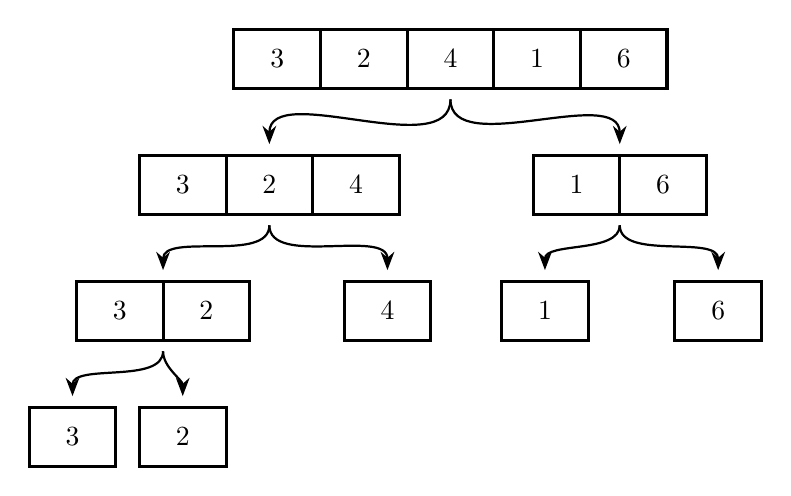
\begin{tikzpicture}[x=1cm,y=1cm,>=Stealth]

% ----- helper: draw array with exact length -----
% \Arr{name}{x}{y}{n}{v1}{v2}{v3}{v4}{v5}
\newcommand{\Arr}[9]{%
  \def\cellW{1.1}\def\H{0.75}
  \coordinate (#1-center) at ({#2 + 0.5*#4*\cellW},{#3 + 0.5*\H});
  \coordinate (#1-north)  at ({#2 + 0.5*#4*\cellW},{#3 + \H});
  \coordinate (#1-south)  at ({#2 + 0.5*#4*\cellW},{#3});
  \draw[line width=1.1pt] (#2,#3) rectangle ({#2 + #4*\cellW}, {#3+\H});
  \foreach \k in {1,...,10} {
    \ifnum\k<#4
      \draw[line width=1.1pt] ({#2+\k*\cellW},#3) -- ({#2+\k*\cellW},{#3+\H});
    \fi
  }
  \ifnum#4>0 \node at ({#2+0.5*\cellW},{#3+0.5*\H}) {#5};\fi
  \ifnum#4>1 \node at ({#2+1.5*\cellW},{#3+0.5*\H}) {#6};\fi
  \ifnum#4>2 \node at ({#2+2.5*\cellW},{#3+0.5*\H}) {#7};\fi
  \ifnum#4>3 \node at ({#2+3.5*\cellW},{#3+0.5*\H}) {#8};\fi
  \ifnum#4>4 \node at ({#2+4.5*\cellW},{#3+0.5*\H}) {#9};\fi
}

% Level 0
\Arr{A0}{3.2}{6.0}{5}{3}{2}{4}{1}{6}

% Level 1 (match video split)
\Arr{L1}{2.0}{4.4}{3}{3}{2}{4}{}{}
\Arr{R1}{7.0}{4.4}{2}{1}{6}{}{}{}

% clean arrows (do not touch boxes)
\draw[->,thick,shorten >=4pt,shorten <=4pt] (A0-south) to[out=-90,in=90] (L1-north);
\draw[->,thick,shorten >=4pt,shorten <=4pt] (A0-south) to[out=-90,in=90] (R1-north);

% Level 2
\Arr{L2a}{1.2}{2.8}{2}{3}{2}{}{}{}
\Arr{L2b}{4.6}{2.8}{1}{4}{}{}{}{}

\Arr{R2a}{6.6}{2.8}{1}{1}{}{}{}{}
\Arr{R2b}{8.8}{2.8}{1}{6}{}{}{}{}

\draw[->,thick,shorten >=4pt,shorten <=4pt] (L1-south) to[out=-90,in=90] (L2a-north);
\draw[->,thick,shorten >=4pt,shorten <=4pt] (L1-south) to[out=-90,in=90] (L2b-north);

\draw[->,thick,shorten >=4pt,shorten <=4pt] (R1-south) to[out=-90,in=90] (R2a-north);
\draw[->,thick,shorten >=4pt,shorten <=4pt] (R1-south) to[out=-90,in=90] (R2b-north);

% -------- ADDITION: split [3,2] into [3] and [2] --------
\Arr{L3a}{0.6}{1.2}{1}{3}{}{}{}{}
\Arr{L3b}{2.0}{1.2}{1}{2}{}{}{}{}

\draw[->,thick,shorten >=4pt,shorten <=4pt] (L2a-south) to[out=-90,in=90] (L3a-north);
\draw[->,thick,shorten >=4pt,shorten <=4pt] (L2a-south) to[out=-90,in=90] (L3b-north);
% --------------------------------------------------------

\end{tikzpicture}
\end{center}

% =========================================================
% Diagram 2: Merge process (ALL steps, like your previous one)
% =========================================================
\subsection{Visualization (Merge)}
We merge sorted halves using three pointers:
$i$ (left), $j$ (right), and $k$ (write index).

% =========================================================
% Merge row for [2,3] | [4] -> out[3]
% =========================================================
\newcommand{\MergeA}[7]{%
\noindent\begin{tikzpicture}[x=1cm,y=1cm,>=Stealth]
  \def\cellW{1.05}\def\H{0.65}

  % L = [2,3]
  \draw[line width=1pt] (0,0) rectangle (2*\cellW,\H);
  \draw[line width=1pt] (\cellW,0) -- (\cellW,\H);
  \node at (0.5*\cellW,0.5*\H) {2};
  \node at (1.5*\cellW,0.5*\H) {3};
  \node[anchor=east] at (-0.25,0.5*\H) {$L$};

  % R = [4]
  \begin{scope}[shift={(3.0,0)}]
    \draw[line width=1pt] (0,0) rectangle (\cellW,\H);
    \node at (0.5*\cellW,0.5*\H) {4};
    \node[anchor=east] at (-0.25,0.5*\H) {$R$};
  \end{scope}

  % out (3 cells)
  \begin{scope}[shift={(5.5,0)}]
    \draw[line width=1pt] (0,0) rectangle (3*\cellW,\H);
    \draw[line width=1pt] (\cellW,0) -- (\cellW,\H);
    \draw[line width=1pt] (2*\cellW,0) -- (2*\cellW,\H);
    \node at (0.5*\cellW,0.5*\H) {#1};
    \node at (1.5*\cellW,0.5*\H) {#2};
    \node at (2.5*\cellW,0.5*\H) {#3};
    \node[anchor=east] at (-0.25,0.5*\H) {$out$};
  \end{scope}

  % pointers
  \ifnum#4>-1
    \draw[->,thick,shorten >=2pt,shorten <=2pt] ({(#4+0.5)*\cellW},1.05) -- ({(#4+0.5)*\cellW},\H);
    \node[anchor=south] at ({(#4+0.5)*\cellW},1.05) {$i$};
  \fi
  \ifnum#5>-1
    \draw[->,thick,shorten >=2pt,shorten <=2pt] ({3.0+(#5+0.5)*\cellW},1.05) -- ({3.0+(#5+0.5)*\cellW},\H);
    \node[anchor=south] at ({3.0+(#5+0.5)*\cellW},1.05) {$j$};
  \fi
  \ifnum#6>-1
    \draw[->,thick,shorten >=2pt,shorten <=2pt] ({5.5+(#6+0.5)*\cellW},1.05) -- ({5.5+(#6+0.5)*\cellW},\H);
    \node[anchor=south] at ({5.5+(#6+0.5)*\cellW},1.05) {$k$};
  \fi

  % caption below
  \node[anchor=west] at (0,-0.35) {#7};
\end{tikzpicture}\par\vspace{0.25cm}
}

% =========================================================
% Merge row for [3] | [2] -> out[2]
% =========================================================
\newcommand{\MergeB}[6]{%
\noindent\begin{tikzpicture}[x=1cm,y=1cm,>=Stealth]
  \def\cellW{1.05}\def\H{0.65}

  % L = [3]
  \draw[line width=1pt] (0,0) rectangle (\cellW,\H);
  \node at (0.5*\cellW,0.5*\H) {3};
  \node[anchor=east] at (-0.25,0.5*\H) {$L$};

  % R = [2]
  \begin{scope}[shift={(2.2,0)}]
    \draw[line width=1pt] (0,0) rectangle (\cellW,\H);
    \node at (0.5*\cellW,0.5*\H) {2};
    \node[anchor=east] at (-0.25,0.5*\H) {$R$};
  \end{scope}

  % out (2)
  \begin{scope}[shift={(4.6,0)}]
    \draw[line width=1pt] (0,0) rectangle (2*\cellW,\H);
    \draw[line width=1pt] (\cellW,0) -- (\cellW,\H);
    \node at (0.5*\cellW,0.5*\H) {#1};
    \node at (1.5*\cellW,0.5*\H) {#2};
    \node[anchor=east] at (-0.25,0.5*\H) {$out$};
  \end{scope}

  % pointers
  \ifnum#3>-1
    \draw[->,thick,shorten >=2pt,shorten <=2pt] ({(#3+0.5)*\cellW},1.05) -- ({(#3+0.5)*\cellW},\H);
    \node[anchor=south] at ({(#3+0.5)*\cellW},1.05) {$i$};
  \fi
  \ifnum#4>-1
    \draw[->,thick,shorten >=2pt,shorten <=2pt] ({2.2+(#4+0.5)*\cellW},1.05) -- ({2.2+(#4+0.5)*\cellW},\H);
    \node[anchor=south] at ({2.2+(#4+0.5)*\cellW},1.05) {$j$};
  \fi
  \ifnum#5>-1
    \draw[->,thick,shorten >=2pt,shorten <=2pt] ({4.6+(#5+0.5)*\cellW},1.05) -- ({4.6+(#5+0.5)*\cellW},\H);
    \node[anchor=south] at ({4.6+(#5+0.5)*\cellW},1.05) {$k$};
  \fi

  % caption below
  \node[anchor=west] at (0,-0.35) {#6};
\end{tikzpicture}\par\vspace{0.25cm}
}

% =========================================================
% Final merge row for [2,3,4] | [1,6] -> out[5]
% =========================================================
\newcommand{\MergeC}[9]{%
\noindent\begin{tikzpicture}[x=1cm,y=1cm,>=Stealth]
  \def\cellW{1.05}\def\H{0.65}
  \def\Rshift{4.4}
  \def\OutShift{8.0}

  % L = [2,3,4]
  \draw[line width=1pt] (0,0) rectangle (3*\cellW,\H);
  \draw[line width=1pt] (\cellW,0) -- (\cellW,\H);
  \draw[line width=1pt] (2*\cellW,0) -- (2*\cellW,\H);
  \node at (0.5*\cellW,0.5*\H) {2};
  \node at (1.5*\cellW,0.5*\H) {3};
  \node at (2.5*\cellW,0.5*\H) {4};
  \node[anchor=east] at (-0.25,0.5*\H) {$L$};

  % R = [1,6]
  \begin{scope}[shift={(\Rshift,0)}]
    \draw[line width=1pt] (0,0) rectangle (2*\cellW,\H);
    \draw[line width=1pt] (\cellW,0) -- (\cellW,\H);
    \node at (0.5*\cellW,0.5*\H) {1};
    \node at (1.5*\cellW,0.5*\H) {6};
    \node[anchor=east] at (-0.25,0.5*\H) {$R$};
  \end{scope}

  % out (5)
  \begin{scope}[shift={(\OutShift,0)}]
    \draw[line width=1pt] (0,0) rectangle (5*\cellW,\H);
    \foreach \t in {1,...,4} { \draw[line width=1pt] (\t*\cellW,0) -- (\t*\cellW,\H); }
    \node at (0.5*\cellW,0.5*\H) {#1};
    \node at (1.5*\cellW,0.5*\H) {#2};
    \node at (2.5*\cellW,0.5*\H) {#3};
    \node at (3.5*\cellW,0.5*\H) {#4};
    \node at (4.5*\cellW,0.5*\H) {#5};
    \node[anchor=east] at (-0.25,0.5*\H) {$out$};
  \end{scope}

  % pointers (hide when index is -1)
  \ifnum#6>-1
    \draw[->,thick,shorten >=2pt,shorten <=2pt] ({(#6+0.5)*\cellW},1.05) -- ({(#6+0.5)*\cellW},\H);
    \node[anchor=south] at ({(#6+0.5)*\cellW},1.05) {$i$};
  \fi

  \ifnum#7>-1
    \draw[->,thick,shorten >=2pt,shorten <=2pt] ({\Rshift+(#7+0.5)*\cellW},1.05) -- ({\Rshift+(#7+0.5)*\cellW},\H);
    \node[anchor=south] at ({\Rshift+(#7+0.5)*\cellW},1.05) {$j$};
  \fi

  \ifnum#8>-1
    \draw[->,thick,shorten >=2pt,shorten <=2pt] ({\OutShift+(#8+0.5)*\cellW},1.05) -- ({\OutShift+(#8+0.5)*\cellW},\H);
    \node[anchor=south] at ({\OutShift+(#8+0.5)*\cellW},1.05) {$k$};
  \fi

  % caption below
  \node[anchor=west] at (0,-0.35) {#9};
\end{tikzpicture}\par\vspace{0.25cm}
}

% =========================================================
% MERGE STEPS
% =========================================================

\textbf{Merge 1:} \([3] \mid [2] \rightarrow [2,3]\)

\MergeB{}{}{0}{0}{0}{Compare 3 vs 2 $\Rightarrow$ write 2}
\MergeB{2}{}{0}{-1}{1}{Right empty $\Rightarrow$ copy left}
\MergeB{2}{3}{-1}{-1}{-1}{Done}

\vspace{0.2cm}

\textbf{Merge 2:} \([2,3] \mid [4] \rightarrow [2,3,4]\)

\MergeA{}{}{}{0}{0}{0}{Compare 2 vs 4 $\Rightarrow$ write 2}
\MergeA{2}{}{}{1}{0}{1}{Compare 3 vs 4 $\Rightarrow$ write 3}
\MergeA{2}{3}{}{-1}{0}{2}{Left empty $\Rightarrow$ copy right}
\MergeA{2}{3}{4}{-1}{-1}{-1}{Done}

\vspace{0.2cm}

\textbf{Merge 3:} \([1] \mid [6] \rightarrow [1,6]\) 

\textbf{Final merge:} \([2,3,4] \mid [1,6] \rightarrow [1,2,3,4,6]\)

\MergeC{}{}{}{}{}{0}{0}{0}{Compare 2 vs 1 $\Rightarrow$ write 1}
\MergeC{1}{}{}{}{}{0}{1}{1}{Compare 2 vs 6 $\Rightarrow$ write 2}
\MergeC{1}{2}{}{}{}{1}{1}{2}{Compare 3 vs 6 $\Rightarrow$ write 3}
\MergeC{1}{2}{3}{}{}{2}{1}{3}{Compare 4 vs 6 $\Rightarrow$ write 4}
\MergeC{1}{2}{3}{4}{}{-1}{1}{4}{Left empty $\Rightarrow$ copy right}
\MergeC{1}{2}{3}{4}{6}{-1}{-1}{-1}{Done}

\subsection{Merge Sort Code (Java)}
\begin{verbatim}
void mergeSort(int[] arr, int s, int e) {
    if (e - s + 1 <= 1) {
        return;   // size <= 1
    }

    int m = (s + e) / 2;
    mergeSort(arr, s, m);       // sort left half
    mergeSort(arr, m + 1, e);   // sort right half

    merge(arr, s, m, e);        // merge sorted halves
}

void merge(int[] arr, int s, int m, int e) {
    int[] L = new int[m - s + 1];
    int[] R = new int[e - m];

    for (int x = 0; x < L.length; x++) {
        L[x] = arr[s + x];
    }
    for (int x = 0; x < R.length; x++) {
        R[x] = arr[m + 1 + x];
    }

    int i = 0;    // pointer for L
    int j = 0;    // pointer for R
    int k = s;    // write pointer for arr

    while (i < L.length && j < R.length) {  // Merge back into arr
        if (L[i] <= R[j]) {
            arr[k] = L[i];
            i++;
        } else {
            arr[k] = R[j];
            j++;
        }
        k++;
    }

    while (i < L.length) {  // Copy remaining from left half
        arr[k] = L[i];
        i++;
        k++;
    }

    while (j < R.length) {  // Copy remaining from right half
        arr[k] = R[j];
        j++;
        k++;
    }
}
\end{verbatim}


\subsection{Time Complexity}
\begin{itemize}
  \item Splitting creates $\log n$ levels (divide by 2 each time)
  \item Each level uses $n$ time to sort
  \item Total: \textbf{$O(n\log n)$}
\end{itemize}

\subsection{Space Complexity}
\begin{itemize}
  \item Temporary arrays during merge: $O(n)$
  \item Recursion depth: $O(\log n)$
  \item Overall extra space: \textbf{$O(n)$}
\end{itemize}
\section{Quicksort}

\textbf{Idea:} Quicksort is a divide-and-conquer algorithm that sorts by
\textbf{partitioning} an array around a chosen pivot.
All elements smaller than the pivot move to the left,
and all elements greater stay on the right.
Then we recursively quicksort the left and right partitions. For simplicity, we choose the \textbf{last element as the pivot}.

% =========================================================
% Visualization (Partition) -- ALL steps
% =========================================================
\subsection{Visualization (Partition)}
Example: \([5,2,4,1,3]\) with pivot = last element (3)

% Usage:
% \QuickStep{a0}{a1}{a2}{a3}{a4}{leftIndex}{iIndex}{note}
% Set iIndex = -1 to hide i (used after loop), set leftIndex = -1 to hide left.
\newcommand{\QuickStep}[8]{%
\noindent\begin{tikzpicture}[x=1cm,y=1cm,>=Stealth]
  \def\n{5}
  \def\cellW{1.25}
  \def\H{0.85}

  % Outer box
  \draw[line width=1.2pt] (0,0) rectangle ({\n*\cellW},\H);

  % Dividers
  \foreach \k in {1,...,4} {
    \draw[line width=1.2pt] ({\k*\cellW},0) -- ({\k*\cellW},\H);
  }

  % Values
  \node at ({0.5*\cellW},0.5*\H) {#1};
  \node at ({1.5*\cellW},0.5*\H) {#2};
  \node at ({2.5*\cellW},0.5*\H) {#3};
  \node at ({3.5*\cellW},0.5*\H) {#4};
  \node at ({4.5*\cellW},0.5*\H) {#5};

  % Pivot pointer (always last index = 4)
  \draw[->,thick] ({(4+0.5)*\cellW},1.70) -- ({(4+0.5)*\cellW},\H);
  \node[anchor=south] at ({(4+0.5)*\cellW},1.70) {$pivot$};

  % If left and i overlap, draw one pointer labeled "left, i"
  \ifnum#6>-1
    \ifnum#7>-1
      \ifnum#6=#7
        \draw[->,thick] ({(#6+0.5)*\cellW},1.45) -- ({(#6+0.5)*\cellW},\H);
        \node[anchor=south] at ({(#6+0.5)*\cellW},1.45) {$left,\ i$};
      \else
        % left pointer (higher)
        \draw[->,thick] ({(#6+0.5)*\cellW},1.60) -- ({(#6+0.5)*\cellW},\H);
        \node[anchor=south] at ({(#6+0.5)*\cellW},1.60) {$left$};

        % i pointer (lower)
        \draw[->,thick] ({(#7+0.5)*\cellW},1.35) -- ({(#7+0.5)*\cellW},\H);
        \node[anchor=south] at ({(#7+0.5)*\cellW},1.35) {$i$};
      \fi
    \else
      % only left shown
      \draw[->,thick] ({(#6+0.5)*\cellW},1.45) -- ({(#6+0.5)*\cellW},\H);
      \node[anchor=south] at ({(#6+0.5)*\cellW},1.45) {$left$};
    \fi
  \else
    % left hidden, maybe i shown
    \ifnum#7>-1
      \draw[->,thick] ({(#7+0.5)*\cellW},1.45) -- ({(#7+0.5)*\cellW},\H);
      \node[anchor=south] at ({(#7+0.5)*\cellW},1.45) {$i$};
    \fi
  \fi

  % Note below
  \node[anchor=west] at (0,-0.45) {#8};
\end{tikzpicture}\par\vspace{0.35cm}
}

% -------------------------
% ALL partition steps
% -------------------------
\QuickStep{5}{2}{4}{1}{3}{0}{0}{Start: $left=0,\ i=0,\ pivot=3$}

\QuickStep{5}{2}{4}{1}{3}{0}{0}{$a[i]=5 > 3 \Rightarrow$ do nothing, $i \leftarrow i+1$}

\QuickStep{5}{2}{4}{1}{3}{0}{1}{$a[i]=2 < 3 \Rightarrow$ swap $a[left]$ and $a[i]$, $left \leftarrow left+1$}

\QuickStep{2}{5}{4}{1}{3}{1}{2}{After swap: $[2,5,4,1,3]$, now $left=1,\ i=2$}

\QuickStep{2}{5}{4}{1}{3}{1}{2}{$a[i]=4 > 3 \Rightarrow$ do nothing, $i \leftarrow i+1$}

\QuickStep{2}{5}{4}{1}{3}{1}{3}{$a[i]=1 < 3 \Rightarrow$ swap $a[left]$ and $a[i]$, $left \leftarrow left+1$}

\QuickStep{2}{1}{4}{5}{3}{2}{-1}{After swap: $[2,1,4,5,3]$, loop ends ($i=e$)}

\QuickStep{2}{1}{4}{5}{3}{2}{-1}{Final step: swap pivot with $a[left]$ (swap $3$ and $4$)}

\QuickStep{2}{1}{3}{5}{4}{2}{-1}{Done partition: pivot placed at index $left$ $\Rightarrow [2,1,3,5,4]$}

After placing the pivot in its correct position, quicksort then sorts the left subarray $[2,1]$ using $1$ as the pivot and the right subarray $[5, 4]$ using $4$ as the pivot, since the previous pivot $3$ is in its final spot. 
% =========================================================
% Code (match the video pseudocode)
% =========================================================
\subsection{Quicksort Code (Java)}
\begin{verbatim}
void quickSort(int[] arr, int s, int e) {
    if (e - s + 1 <= 1) return;

    int pivot = arr[e];
    int left = s;

    // partition
    for (int i = s; i < e; i++) {
        if (arr[i] < pivot) {
            int temp = arr[left];
            arr[left] = arr[i];
            arr[i] = temp;
            left++;
        }
    }

    // move pivot between the partitions
    int temp = arr[left];
    arr[left] = arr[e];
    arr[e] = temp;

    // recurse on left and right partitions
    quickSort(arr, s, left - 1);
    quickSort(arr, left + 1, e);
}
\end{verbatim}

\subsection{Time Complexity}
\begin{itemize}
  \item \textbf{Best case:} $O(n\log n)$ (pivot splits evenly)
  \item \textbf{Average case:} $O(n\log n)$
  \item \textbf{Worst case:} $O(n^2)$ (pivot gives very unbalanced splits)
\end{itemize}

\subsection{Space Complexity}
\begin{itemize}
  \item In-place partitioning uses $O(1)$ extra array space
  \item Recursion stack: $O(\log n)$ average, $O(n)$ worst
\end{itemize}
\section{Binary Search Trees}

\subsection{Binary Trees}

A \textbf{tree} is a hierarchical data structure made of \textbf{nodes} connected by edges/pointers.  
Unlike arrays or linked lists, trees do not store data linearly. Instead, they branch.

Each node contains:
\begin{itemize}
  \item a value
  \item a reference to a left child (optional)
  \item a reference to a right child (optional)
\end{itemize}

\textbf{Binary trees} restrict each node to at most two children.

\textbf{Tree terminology:}
\begin{itemize}
  \item \textbf{Root}: the topmost node
  \item \textbf{Parent}: a node that points to children
  \item \textbf{Child}: a node pointed to by a parent
  \item \textbf{Leaf}: a node with no children
  \item \textbf{Depth}: number of edges from the root to a node
  \item \textbf{Height}: number of edges in the longest path from a node to a leaf
\end{itemize}

\subsection{Binary Search Trees}

A \textbf{Binary Search Tree (BST)} is a binary tree with a \textbf{sorted property}:

\begin{itemize}
  \item For \textbf{every node}, all values in its left subtree are \textbf{less than} the node's value
  \item For \textbf{every node}, all values in its right subtree are \textbf{greater than} the node's value
\end{itemize}

This property makes a BST behave like a sorted array, allowing us to eliminate half of the tree at every step during search. 

Assuming that a BST is perfectly balanced, searching, inserting and deleting are all $O(\log n)$ operations. Meanwhile, arrays require $O(n)$ shifts for insert/delete.

\begin{center}
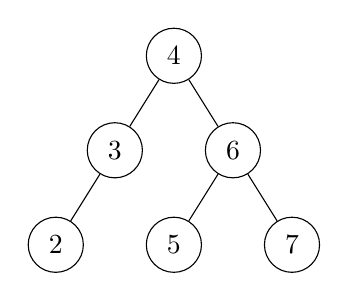
\begin{tikzpicture}[
  level distance=1.2cm,
  every node/.style={circle, draw, minimum size=7mm},
  edge from parent/.style={draw,-}
]
\node {4}
  child { node {3}
    child { node {2} }
    child[missing] {}
  }
  child { node {6}
    child { node {5} }
    child { node {7} }
  };
\end{tikzpicture}
\end{center}

\subsection{BST Search (Recursive)}

Searching in a balanced BST has a time complexity of \textbf{$O(\log n)$} while searching in a unbalanced tree is $O(n)$ as it's essentially been degenerated into a linked list.

\textbf{Example: search for 5}

\begin{center}
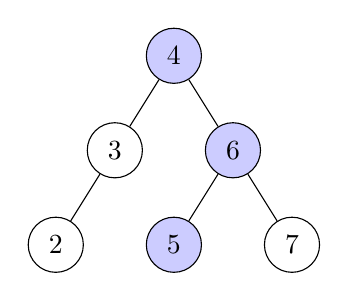
\begin{tikzpicture}[
  level distance=1.2cm,
  every node/.style={circle, draw, minimum size=7mm},
  edge from parent/.style={draw,-},
  highlight/.style={circle, draw, fill=blue!20}
]
\node[highlight] {4}
  child { node {3}
    child { node {2} }
    child[missing] {}
  }
  child { node[highlight] {6}
    child { node[highlight] {5} }
    child { node {7} }
  };
\end{tikzpicture}
\end{center}

Path: $4 \rightarrow 6 \rightarrow 5$

\begin{verbatim}
boolean search(TreeNode root, int target) {
    if (root == null) return false;
    if (root.val == target) return true;
    if (target < root.val) return search(root.left, target);
    else return search(root.right, target);
}
\end{verbatim}

\subsection{Insertion in a BST}

Insertion follows the same logic as search:
\begin{itemize}
  \item If value is smaller, go left
  \item If value is larger, go right
  \item Insert when you hit a null pointer
\end{itemize}

\textbf{Example: insert 1}

\begin{center}
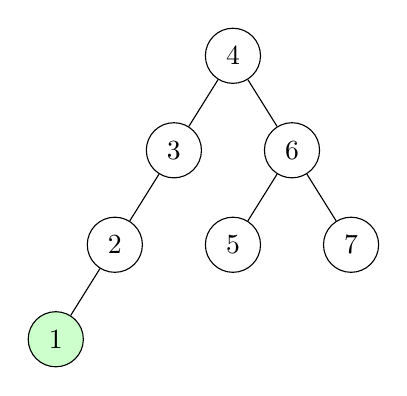
\begin{tikzpicture}[
  level distance=1.2cm,
  every node/.style={circle, draw, minimum size=7mm},
  edge from parent/.style={draw,-},
  new/.style={circle, draw, fill=green!20}
]
\node {4}
  child { node {3}
    child { node {2}
      child { node[new] {1} }
      child[missing] {}
    }
    child[missing] {}
  }
  child { node {6}
    child { node {5} }
    child { node {7} }
  };
\end{tikzpicture}
\end{center}

\begin{verbatim}
TreeNode insert(TreeNode root, int val) {
    if (root == null) return new TreeNode(val);
    if (val < root.val)
        root.left = insert(root.left, val);
    else
        root.right = insert(root.right, val);
    return root;
}
\end{verbatim}

\subsection{Finding the Minimum Value}

The minimum value in a BST is found by going left until we cannot go further.

\begin{center}
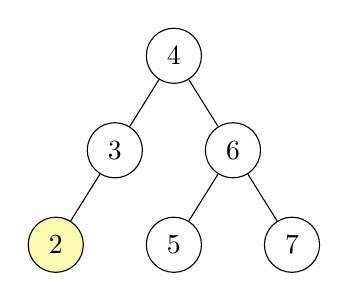
\begin{tikzpicture}[
  level distance=1.2cm,
  every node/.style={circle, draw, minimum size=7mm},
  edge from parent/.style={draw,-},
  highlight/.style={circle, draw, fill=yellow!30}
]
\node {4}
  child { node {3}
    child { node[highlight] {2} }
    child[missing] {}
  }
  child { node {6}
    child { node {5} }
    child { node {7} }
  };
\end{tikzpicture}
\end{center}

\begin{verbatim}
TreeNode findMin(TreeNode root) {
    while (root.left != null)
        root = root.left;
    return root;
}
\end{verbatim}
\subsection{Deleting a Node in a BST}

We use the same example tree throughout:

\begin{center}
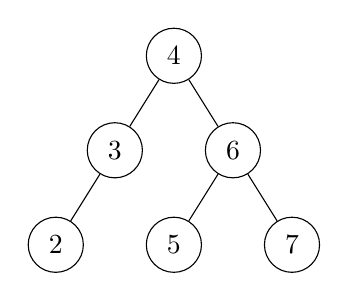
\begin{tikzpicture}[
  level distance=1.2cm,
  every node/.style={circle, draw, minimum size=7mm},
  edge from parent/.style={draw,-}
]
\node {4}
  child { node {3}
    child { node {2} }
    child[missing] {}
  }
  child { node {6}
    child { node {5} }
    child { node {7} }
  };
\end{tikzpicture}
\end{center}

\textbf{Case 1: Leaf node (no children)}  

Example: delete node 2

\begin{center}
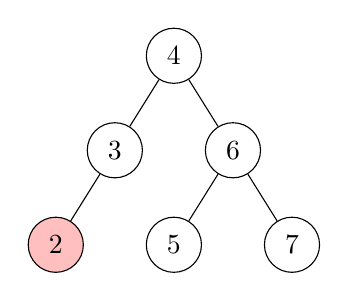
\begin{tikzpicture}[
  level distance=1.2cm,
  every node/.style={circle, draw, minimum size=7mm},
  edge from parent/.style={draw,-},
  removed/.style={circle, draw, fill=red!25}
]
\node {4}
  child { node {3}
    child { node[removed] {2} }
    child[missing] {}
  }
  child { node {6}
    child { node {5} }
    child { node {7} }
  };
\end{tikzpicture}
\end{center}

Node 2 is simply removed and replaced with \texttt{null}.

\bigskip

\textbf{Case 2: Node with one child}  

Example: delete node 3

Return the non-null child.

\begin{center}
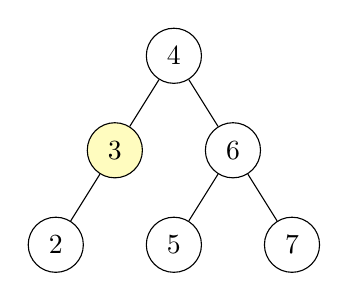
\begin{tikzpicture}[
  level distance=1.2cm,
  every node/.style={circle, draw, minimum size=7mm},
  edge from parent/.style={draw,-},
  highlight/.style={circle, draw, fill=yellow!25}
]



\node {4}
  child { node[highlight] {3}
    child { node {2} }
    child[missing] {}
  }
  child { node {6}
    child { node {5} }
    child { node {7} }
  };
\end{tikzpicture}
\end{center}

After deletion, node 2 moves up to replace node 3.

\bigskip

\textbf{Case 3: Node with two children}  

\textbf{Example: delete node 4}

Replace the node to remove with the smallest leaf node in the right subtree or the largest leaf node in the left subtree. Then delete that leaf.


\textbf{Step 1: find successor}

\begin{center}
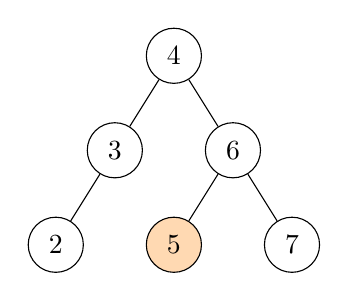
\begin{tikzpicture}[
  level distance=1.2cm,
  every node/.style={circle, draw, minimum size=7mm},
  edge from parent/.style={draw,-},
  highlight/.style={circle, draw, fill=orange!30}
]
\node {4}
  child { node {3}
    child { node {2} }
    child[missing] {}
  }
  child { node {6}
    child { node[highlight] {5} }
    child { node {7} }
  };
\end{tikzpicture}
\end{center}

\textbf{Step 2: replace and delete leaf}

\begin{center}
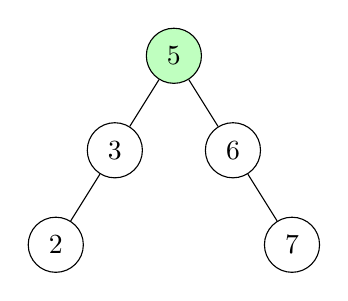
\begin{tikzpicture}[
  level distance=1.2cm,
  every node/.style={circle, draw, minimum size=7mm},
  edge from parent/.style={draw,-},
  newroot/.style={circle, draw, fill=green!25}
]
\node[newroot] {5}
  child { node {3}
    child { node {2} }
    child[missing] {}
  }
  child { node {6}
    child[missing] {}
    child { node {7} }
  };
\end{tikzpicture}
\end{center}

\begin{verbatim}
TreeNode deleteNode(TreeNode root, int key) {
    if (root == null) return null;
    if (key < root.val)
        root.left = deleteNode(root.left, key);
    else if (key > root.val)
        root.right = deleteNode(root.right, key);
    else {
        if (root.left == null) return root.right;
        if (root.right == null) return root.left;
        TreeNode minNode = findMin(root.right);
        root.val = minNode.val;
        root.right = deleteNode(root.right, minNode.val);
    }
    return root;
}
\end{verbatim}


\subsection{Depth-First Search (DFS)}

Depth-first search explores a tree by going as deep as possible before backtracking.  
All traversals below use the following tree:

\begin{center}
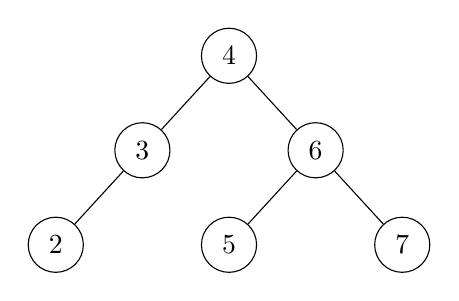
\begin{tikzpicture}[
  level distance=1.2cm,
  sibling distance=2.2cm,
  every node/.style={circle, draw, minimum size=7mm},
  edge from parent/.style={draw,-}
]
\node {4}
  child { node {3}
    child { node {2} }
    child[missing] {}
  }
  child { node {6}
    child { node {5} }
    child { node {7} }
  };
\end{tikzpicture}
\end{center}

There are three common DFS traversal orders:

\textbf{Inorder (left $\rightarrow$ root $\rightarrow$ right)}  
Prints values in sorted order for a BST:
\[
2, 3, 4, 5, 6, 7
\]

\begin{verbatim}
void inorder(TreeNode root) {
    if (root == null) return;
    inorder(root.left);
    System.out.print(root.val + " ");
    inorder(root.right);
}
\end{verbatim}

\textbf{Preorder (root $\rightarrow$ left $\rightarrow$ right)}  
Processes the root before its subtrees (useful for copying/serialization):
\[
4, 3, 2, 6, 5, 7
\]

\begin{verbatim}
void preorder(TreeNode root) {
    if (root == null) return;
    System.out.print(root.val + " ");
    preorder(root.left);
    preorder(root.right);
}
\end{verbatim}

\textbf{Postorder (left $\rightarrow$ right $\rightarrow$ root)}  
Processes children before the parent (useful for deletion/evaluation):
\[
2, 3, 5, 7, 6, 4
\]

\begin{verbatim}
void postorder(TreeNode root) {
    if (root == null) return;
    postorder(root.left);
    postorder(root.right);
    System.out.print(root.val + " ");
}
\end{verbatim}

\subsection{Breadth-First Search (BFS)}

Breadth-first search visits nodes \textbf{level by level}, from top to bottom and left to right.

Using the same tree, BFS prints:
\[
4 \rightarrow 3,6 \rightarrow 2,5,7
\]

BFS uses a \textbf{queue (FIFO)} because nodes are processed in the order they are discovered.

\begin{verbatim}
void bfs(TreeNode root) {
    if (root == null){
        return;
    }

    Queue<TreeNode> q = new LinkedList<>();
    q.add(root);

    while (!q.isEmpty()) {
        TreeNode curr = q.peek();
        System.out.print(curr.val + " ");
        q.remove();

        if (curr.left != null) q.add(curr.left);
        if (curr.right != null) q.add(curr.right);
    }
}
\end{verbatim}

\textbf{Time Complexity:} $O(n)$  
Each node is visited exactly once.
\section{Hash Maps}

A \textbf{hash map} stores \textbf{(key, value)} pairs and supports fast lookup by key.  
In a hash map, insert/search/remove are \textbf{$O(1)$}. Hash maps do \textbf{not maintain any order}, so the physical placement of keys in the table has no relation to insertion order or sorted order.

\subsection{Core Idea}
A hash map is implemented using an \textbf{array}. 
A \textbf{hash function} converts a key into an integer index:
\[
\text{index} = h(\text{key}) \bmod m
\]
where $m$ is the table size.

The same key always hashes to the same index.

\subsection{Example Hash Function}
An example of a hash function for strings:
\begin{itemize}
  \item sum ASCII values of characters
  \item mod by table size to stay in bounds
\end{itemize}

\begin{verbatim}
int hash(String key, int tableSize) {
    int sum = 0;
    for (char c : key.toCharArray()) {
        sum += c;
    }
    return sum % tableSize;
}
\end{verbatim}

\subsection{Step-by-Step Insertion Example (Open Addressing)}

Initial table size: $m = 2$ (indices 0 and 1)

\begin{center}
\begin{tabular}{c c}
\toprule
Index & Value \\
\midrule
0 & -- \\
1 & -- \\
\bottomrule
\end{tabular}
\end{center}

\textbf{Insert:} \texttt{("Alice", "NYC")}  
Assume $\text{hash(Alice)} = 25 \Rightarrow 25 \bmod 2 = 1$

\begin{center}
\begin{tabular}{c c}
\toprule
Index & Value \\
\midrule
0 & -- \\
1 & (Alice, NYC) \\
\bottomrule
\end{tabular}
\end{center}

The table is now half full $\Rightarrow$ \textbf{resize and rehash}. We do this to reduce collisions, keeping insert, search, and remove $O(1)$ time.

\subsection{Rehashing (after resize to size 4)}
Recompute all indices using new size $m = 4$.

\[
25 \bmod 4 = 1
\]

\begin{center}
\begin{tabular}{c c}
\toprule
Index & Value \\
\midrule
0 & -- \\
1 & (Alice, NYC) \\
2 & -- \\
3 & -- \\
\bottomrule
\end{tabular}
\end{center}

\textbf{Insert:} \texttt{("Brad", "Chicago")}  
Assume hash = 27, $27 \bmod 4 = 3$

\begin{center}
\begin{tabular}{c c}
\toprule
Index & Value \\
\midrule
0 & -- \\
1 & (Alice, NYC) \\
2 & -- \\
3 & (Brad, Chicago) \\
\bottomrule
\end{tabular}
\end{center}

The table is now half full again $\Rightarrow$ \textbf{resize and rehash}.  

\subsection{Rehashing (after resize to size 8)}
Recompute all indices using new size $m = 8$.

\[
25 \bmod 8 = 1,\quad 27 \bmod 8 = 3
\]

\begin{center}
\begin{tabular}{c c}
\toprule
Index & Value \\
\midrule
0 & -- \\
1 & (Alice, NYC) \\
2 & -- \\
3 & (Brad, Chicago) \\
4 & -- \\
5 & -- \\
6 & -- \\
7 & -- \\
\bottomrule
\end{tabular}
\end{center}

\subsection{Collision Example (Open Addressing)}
\textbf{Insert:} \texttt{("Collin", "Seattle")}  
Assume hash = 33, $33 \bmod 8 = 1$ $\Rightarrow$ collision with Alice. In this example, we handle collisions with \textbf{open addressing}, where we find the next empty slot in the array so that multiple keys can still be stored even when they hash to the same index. Other collision-handling strategies exist, such as \textbf{chaining}, where each index stores a linked list of key–value pairs instead of using probing.


\begin{itemize}
  \item index 1 is occupied
  \item try index 2 (empty)
\end{itemize}

\begin{center}
\begin{tabular}{c c}
\toprule
Index & Value \\
\midrule
0 & -- \\
1 & (Alice, NYC) \\
2 & (Collin, Seattle) \\
3 & (Brad, Chicago) \\
4 & -- \\
5 & -- \\
6 & -- \\
7 & -- \\
\bottomrule
\end{tabular}
\end{center}

\subsection{Search Example (After Collision)}

Because collisions push elements forward, search must also \textbf{probe forward} until the key is found or an empty slot is reached.

\begin{verbatim}
get(key):
    index = h(key) % m
    while table[index] is not empty:
        if table[index].key == key:
            return table[index].value
        index = (index + 1) % m   // linear probing
    return NOT_FOUND
\end{verbatim}

\subsubsection*{Example 1: Key Found}
Search for \texttt{"Collin"}:

\begin{itemize}
  \item hash("Collin") = 33 $\Rightarrow 33 \bmod 8 = 1$
  \item index 1 contains Alice $\Rightarrow$ not a match
  \item probe next index (2)
  \item index 2 contains Collin $\Rightarrow$ found
\end{itemize}

\[
\text{get("Collin")} = \text{"Seattle"}
\]

\subsubsection*{Example 2: Key Not Found}
Search for \texttt{"Daniel"} (assume it also hashes to index 1 for this example):

\begin{itemize}
  \item start at index 1
  \item index 1: Alice (not match)
  \item index 2: Collin (not match)
  \item index 3: Brad (not match)
  \item index 4: empty slot reached $\Rightarrow$ stop
\end{itemize}

\[
\text{get("Daniel")} = \text{NOT\_FOUND}
\]

Reaching an empty slot means the key does not exist, since insertion would have stopped there.

\subsection{Duplicate Key (Overwrite)}
Keys are typically \textbf{unique} (no duplicate keys). Inserting an existing key usually \textbf{overwrites} its value.

Insert \texttt{("Alice", "Boston")}:

\begin{itemize}
  \item hash gives index 1
  \item key already exists
  \item value is overwritten
\end{itemize}

\begin{center}
\begin{tabular}{c c}
\toprule
Index & Value \\
\midrule
0 & -- \\
1 & (Alice, Boston) \\
2 & (Collin, Seattle) \\
3 & (Brad, Chicago) \\
4 & -- \\
5 & -- \\
6 & -- \\
7 & -- \\
\bottomrule
\end{tabular}
\end{center}

\subsection{Deletion + Tombstones (Open Addressing)}
With open addressing, we \textbf{cannot} delete by setting a slot to empty (\texttt{--}), because that can break the probe chain and cause searches to stop early.  
Instead, we mark deleted slots with a \textbf{tombstone} (e.g. \texttt{DEL}).

\subsubsection*{Tombstone Example}
\textbf{Remove:} \texttt{"Brad"} (at index 3) $\Rightarrow$ mark as \texttt{DEL} (tombstone), not empty.

\begin{center}
\begin{tabular}{c c}
\toprule
Index & Value \\
\midrule
0 & -- \\
1 & (Alice, Boston) \\
2 & (Collin, Seattle) \\
3 & DEL \\
4 & -- \\
5 & -- \\
6 & -- \\
7 & -- \\
\bottomrule
\end{tabular}
\end{center}

\textbf{How search changes:}
\begin{itemize}
  \item \texttt{DEL} means ``keep probing'' (key might be later in the chain)
  \item \texttt{--} means ``stop'' (key does not exist)
\end{itemize}

\textbf{How insert changes:}
\begin{itemize}
  \item \texttt{DEL} can be reused as an insertion spot
\end{itemize}

\begin{verbatim}
get(key):
    idx = h(key) % m
    while table[idx] != EMPTY:
        if table[idx] != DEL and table[idx].key == key:
            return table[idx].value
        idx = (idx + 1) % m
    return NOT_FOUND
\end{verbatim}

\subsection{Time Complexity}

\begin{center}
\begin{tabular}{l c c}
\toprule
\textbf{Operation} & \textbf{Average Case} & \textbf{Worst Case} \\
\midrule
Insert & $O(1)$ & $O(n)$ \\
Search & $O(1)$ & $O(n)$ \\
Remove & $O(1)$ & $O(n)$ \\
\bottomrule
\end{tabular}
\end{center}

Worst case happens when many keys collide, forcing long probing/chains, but this is very unlikely with a good hash function and regular resizing.
\input{sections/11-binary-search-trees}
\section{Backtracking}

Backtracking is a DFS-based algorithmic technique where we try all possible paths
and \textbf{backtrack} (undo choices) when we hit a dead-end.


\subsection{Q1: Determine if a valid root-to-leaf path exists}

\textbf{Q:} Determine if a path exists from the root to a leaf node such that no node in the path contains $0$.

\begin{verbatim}
boolean canReachLeaf(TreeNode root) {
    if (root == null || root.val == 0) return false;

    if (root.left == null && root.right == null)
        return true;

    if (canReachLeaf(root.left)) return true;
    if (canReachLeaf(root.right)) return true;

    return false;
}
\end{verbatim}

\textbf{Step-by-step traversal:}

\begin{center}
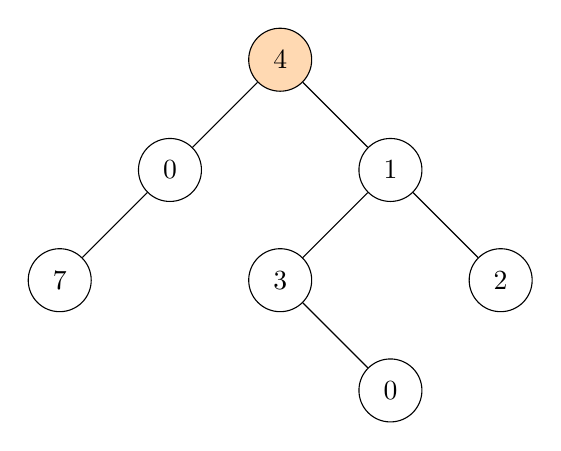
\begin{tikzpicture}[
  level distance=1.4cm,
  sibling distance=2.8cm,
  every node/.style={circle, draw, minimum size=8mm},
  edge from parent/.style={draw,-},
  curr/.style={circle, draw, fill=orange!30}
]
\node[curr] {4}
  child { node {0}
    child { node {7} }
    child[missing] {}
  }
  child { node {1}
    child { node {3}
      child[missing] {}
      child { node {0} }
    }
    child { node {2} }
  };
\end{tikzpicture}

{\small Start at root (4)}
\end{center}

\begin{center}
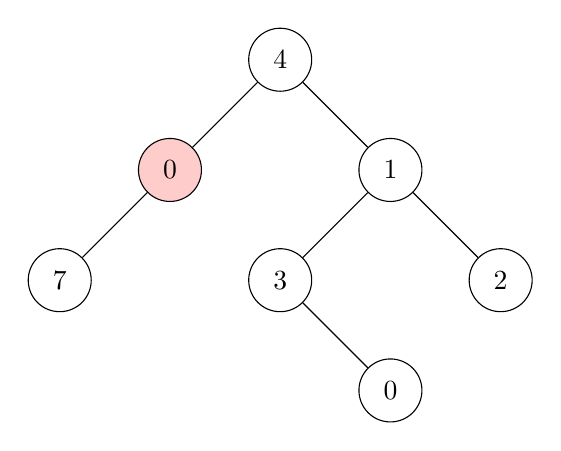
\begin{tikzpicture}[
  level distance=1.4cm,
  sibling distance=2.8cm,
  every node/.style={circle, draw, minimum size=8mm},
  edge from parent/.style={draw,-},
  bad/.style={circle, draw, fill=red!20}
]
\node {4}
  child { node[bad] {0}
    child { node {7} }
    child[missing] {}
  }
  child { node {1}
    child { node {3}
      child[missing] {}
      child { node {0} }
    }
    child { node {2} }
  };
\end{tikzpicture}

{\small Left subtree fails (contains 0), return false $\Rightarrow$ backtrack}
\end{center}

\begin{center}
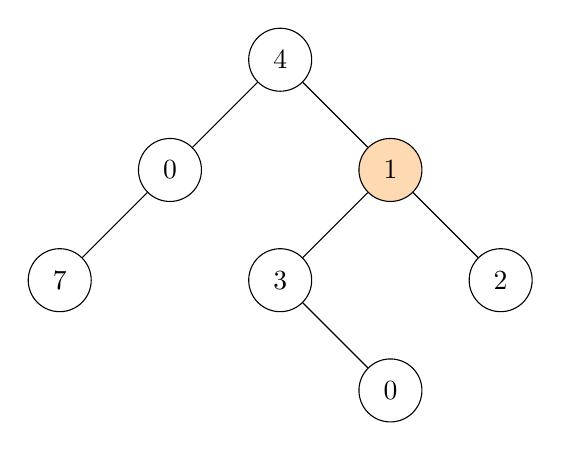
\begin{tikzpicture}[
  level distance=1.4cm,
  sibling distance=2.8cm,
  every node/.style={circle, draw, minimum size=8mm},
  edge from parent/.style={draw,-},
  curr/.style={circle, draw, fill=orange!30}
]
\node {4}
  child { node {0}
    child { node {7} }
    child[missing] {}
  }
  child { node[curr] {1}
    child { node {3}
      child[missing] {}
      child { node {0} }
    }
    child { node {2} }
  };
\end{tikzpicture}

{\small Move to right subtree (node 1)}
\end{center}

\begin{center}
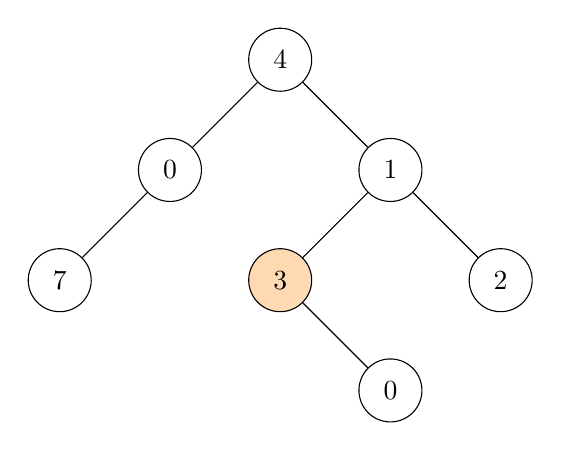
\begin{tikzpicture}[
  level distance=1.4cm,
  sibling distance=2.8cm,
  every node/.style={circle, draw, minimum size=8mm},
  edge from parent/.style={draw,-},
  curr/.style={circle, draw, fill=orange!30}
]
\node {4}
  child { node {0}
    child { node {7} }
    child[missing] {}
  }
  child { node {1}
    child { node[curr] {3}
      child[missing] {}
      child { node {0} }
    }
    child { node {2} }
  };
\end{tikzpicture}

{\small Explore left subtree first (node 3)}
\end{center}

\begin{center}
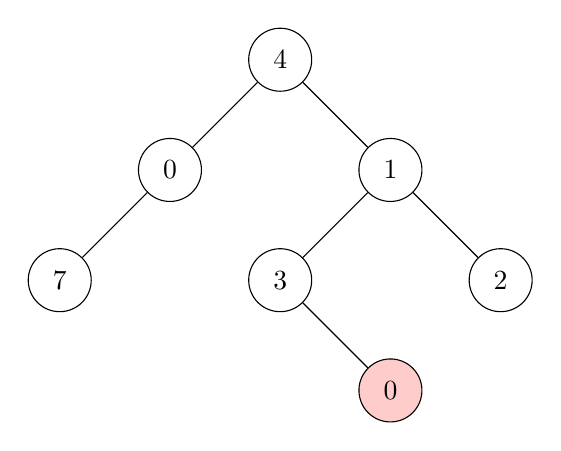
\begin{tikzpicture}[
  level distance=1.4cm,
  sibling distance=2.8cm,
  every node/.style={circle, draw, minimum size=8mm},
  edge from parent/.style={draw,-},
  bad/.style={circle, draw, fill=red!20}
]
\node {4}
  child { node {0}
    child { node {7} }
    child[missing] {}
  }
  child { node {1}
    child { node {3}
      child[missing] {}
      child { node[bad] {0} }
    }
    child { node {2} }
  };
\end{tikzpicture}

{\small Node 3's child is 0 (invalid), return false $\Rightarrow$ backtrack to node 1}
\end{center}

\begin{center}
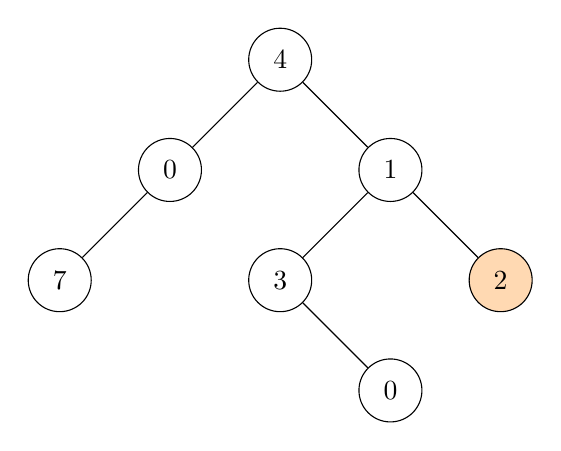
\begin{tikzpicture}[
  level distance=1.4cm,
  sibling distance=2.8cm,
  every node/.style={circle, draw, minimum size=8mm},
  edge from parent/.style={draw,-},
  curr/.style={circle, draw, fill=orange!30}
]
\node {4}
  child { node {0}
    child { node {7} }
    child[missing] {}
  }
  child { node {1}
    child { node {3}
      child[missing] {}
      child { node {0} }
    }
    child { node[curr] {2} }
  };
\end{tikzpicture}

{\small Check node 2 (leaf) — valid path found}
\end{center}

Valid path:
\[
4 \rightarrow 1 \rightarrow 2
\]

% =========================================================
\subsection{Q2: Build the path using backtracking}

Now we must build the path and remove nodes when a branch fails.

\begin{verbatim}
boolean leafPath(TreeNode root, List<Integer> path) {
    if (root == null || root.val == 0) return false;

    path.add(root.val);

    if (root.left == null && root.right == null)
        return true;

    if (leafPath(root.left, path)) return true;
    if (leafPath(root.right, path)) return true;

    path.remove(path.size() - 1);   // backtrack
    return false;
}
\end{verbatim}

\textbf{Step-by-step with live path updates:}

\begin{center}
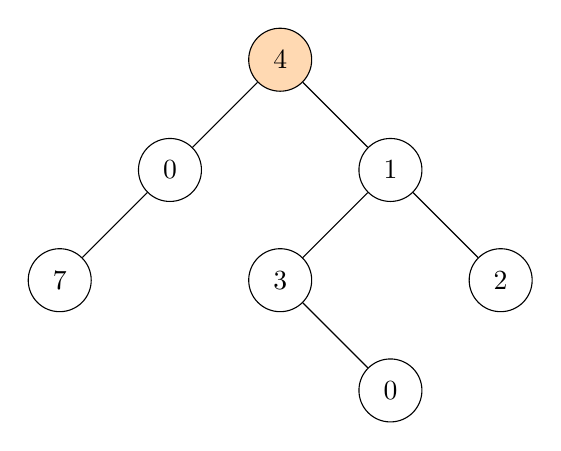
\begin{tikzpicture}[
  level distance=1.4cm,
  sibling distance=2.8cm,
  every node/.style={circle, draw, minimum size=8mm},
  edge from parent/.style={draw,-},
  curr/.style={circle, draw, fill=orange!30}
]
\node[curr] {4}
  child { node {0}
    child { node {7} }
    child[missing] {}
  }
  child { node {1}
    child { node {3}
      child[missing] {}
      child { node {0} }
    }
    child { node {2} }
  };
\end{tikzpicture}

{\small Path = [4]}
\end{center}

\begin{center}
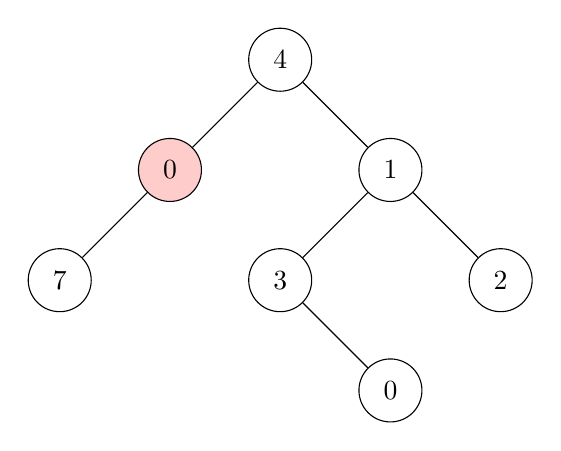
\begin{tikzpicture}[
  level distance=1.4cm,
  sibling distance=2.8cm,
  every node/.style={circle, draw, minimum size=8mm},
  edge from parent/.style={draw,-},
  bad/.style={circle, draw, fill=red!20}
]
\node {4}
  child { node[bad] {0}
    child { node {7} }
    child[missing] {}
  }
  child { node {1}
    child { node {3}
      child[missing] {}
      child { node {0} }
    }
    child { node {2} }
  };
\end{tikzpicture}

{\small Go left: hit 0 (invalid), path unchanged}
\end{center}

\begin{center}
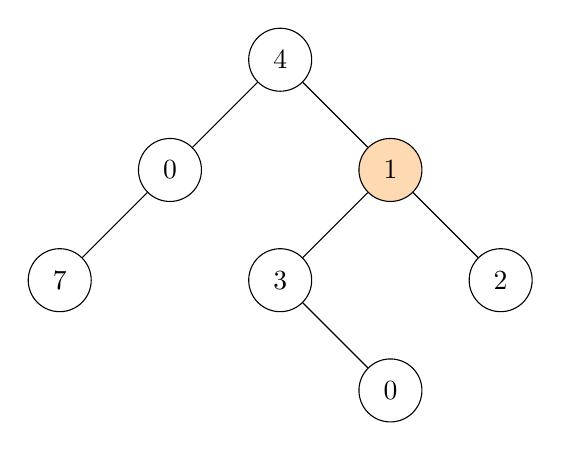
\begin{tikzpicture}[
  level distance=1.4cm,
  sibling distance=2.8cm,
  every node/.style={circle, draw, minimum size=8mm},
  edge from parent/.style={draw,-},
  curr/.style={circle, draw, fill=orange!30}
]
\node {4}
  child { node {0}
    child { node {7} }
    child[missing] {}
  }
  child { node[curr] {1}
    child { node {3}
      child[missing] {}
      child { node {0} }
    }
    child { node {2} }
  };
\end{tikzpicture}

{\small Path = [4, 1]}
\end{center}

\begin{center}
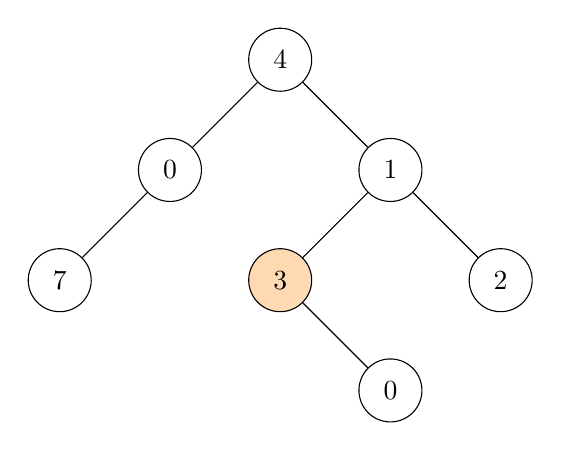
\begin{tikzpicture}[
  level distance=1.4cm,
  sibling distance=2.8cm,
  every node/.style={circle, draw, minimum size=8mm},
  edge from parent/.style={draw,-},
  curr/.style={circle, draw, fill=orange!30}
]
\node {4}
  child { node {0}
    child { node {7} }
    child[missing] {}
  }
  child { node {1}
    child { node[curr] {3}
      child[missing] {}
      child { node {0} }
    }
    child { node {2} }
  };
\end{tikzpicture}

{\small Path = [4, 1, 3]}
\end{center}

\begin{center}
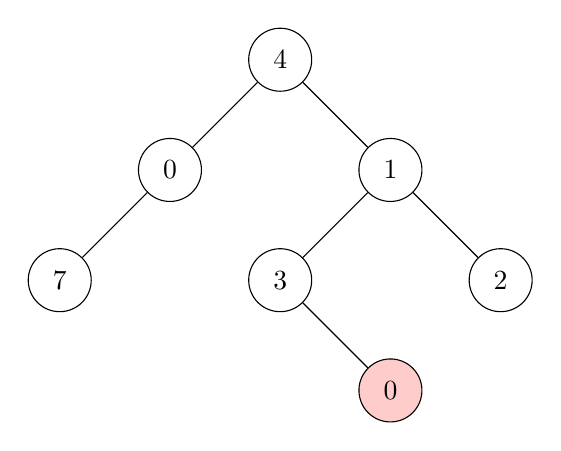
\begin{tikzpicture}[
  level distance=1.4cm,
  sibling distance=2.8cm,
  every node/.style={circle, draw, minimum size=8mm},
  edge from parent/.style={draw,-},
  bad/.style={circle, draw, fill=red!20}
]
\node {4}
  child { node {0}
    child { node {7} }
    child[missing] {}
  }
  child { node {1}
    child { node {3}
      child[missing] {}
      child { node[bad] {0} }
    }
    child { node {2} }
  };
\end{tikzpicture}

{\small From node 3, child is 0 (invalid) $\Rightarrow$ backtrack, pop 3}
\end{center}

\begin{center}
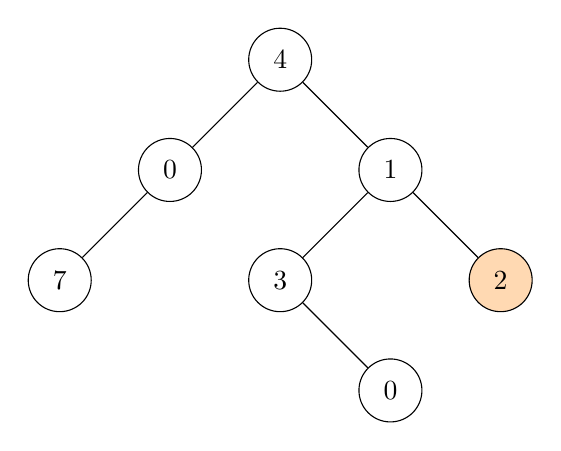
\begin{tikzpicture}[
  level distance=1.4cm,
  sibling distance=2.8cm,
  every node/.style={circle, draw, minimum size=8mm},
  edge from parent/.style={draw,-},
  curr/.style={circle, draw, fill=orange!30}
]
\node {4}
  child { node {0}
    child { node {7} }
    child[missing] {}
  }
  child { node {1}
    child { node {3}
      child[missing] {}
      child { node {0} }
    }
    child { node[curr] {2} }
  };
\end{tikzpicture}

{\small Path = [4, 1, 2] (leaf)}
\end{center}

Final path:
\[
[4, 1, 2]
\]

\subsection{Time and Space Complexity}
\begin{itemize}
  \item \textbf{Time:} $O(n)$ — may visit all nodes
  \item \textbf{Space:} $O(h)$ — recursion depth and path length
\end{itemize}
\section{Heaps / Priority Queue}

A \textbf{heap} is a specialized tree-based data structure used to implement a \textbf{priority queue}.  
The goal of a heap is to always be able to access the \textbf{minimum or maximum value in $O(1)$} time.

\begin{itemize}
  \item A \textbf{min-heap} stores the smallest value at the root
  \item A \textbf{max-heap} stores the largest value at the root
\end{itemize}

In this section, we focus on \textbf{min-heaps}. Max-heaps work the same way with reversed comparisons.

\subsection{Heap Properties}

A binary tree is a heap if it satisfies the following two properties:

\subsubsection*{1. Structure Property (Complete Binary Tree)}
\begin{itemize}
  \item There are \textbf{no holes} in the tree (All levels are completely filled except possibly the last)
  \item The last level must be filled \textbf{from left to right}
\end{itemize}

\subsubsection*{2. Order Property (Min-Heap)}
For \textbf{every node}, all of its descendants must be \textbf{greater than or equal to} that node.  
This guarantees the minimum value is always at the root.

\subsection{Array Representation}

Although we draw heaps as trees, they are stored in an \textbf{array} using \textbf{level-order (BFS)} traversal.  
We ignore index 0 and store the root at index 1 so the math works cleanly:

\[
\text{left} = 2i, \quad \text{right} = 2i + 1, \quad \text{parent} = \left\lfloor \frac{i}{2} \right\rfloor
\]

\[
[\text{EMPTY},\ 14,\ 19,\ 16,\ 21,\ 26,\ 19,\ 68,\ 65,\ 30]
\]

\subsection{Push (Insert) --- Example: Insert 17}

To push into a heap:
\begin{itemize}
  \item Insert at the end of the array (next open spot)
  \item Percolate up: Repeatedly swap the new value with its parent while it is smaller, moving it upward until its parent is smaller than or equal to it.
\end{itemize}

\textbf{Step 1: Starting heap}

\[
[\text{EMPTY},\ 14,\ 19,\ 16,\ 21,\ 26,\ 19,\ 68,\ 65,\ 30]
\]

\begin{center}
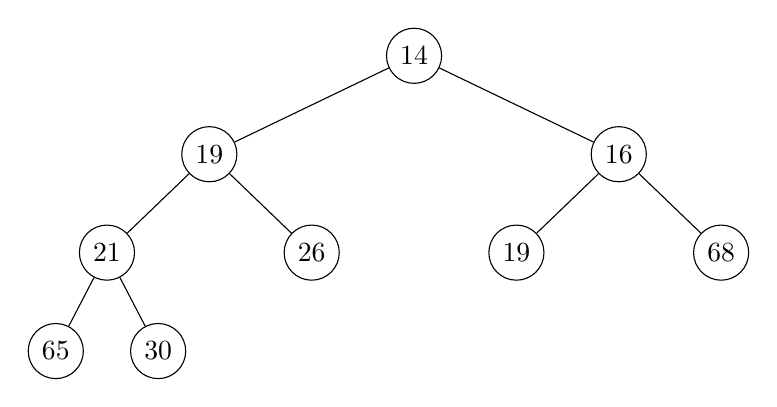
\begin{tikzpicture}[
  level distance=1.25cm,
  level 1/.style={sibling distance=5.2cm},
  level 2/.style={sibling distance=2.6cm},
  level 3/.style={sibling distance=1.3cm},
  every node/.style={circle, draw, minimum size=7mm, inner sep=1pt},
  edge from parent/.style={draw,-}
]
\node {14}
  child { node {19}
    child { node {21}
      child { node {65} }
      child { node {30} }
    }
    child { node {26} }
  }
  child { node {16}
    child { node {19} }
    child { node {68} }
  };
\end{tikzpicture}
\end{center}

\textbf{Step 2: append 17 at index 10}

\[
[\text{EMPTY},\ 14,\ 19,\ 16,\ 21,\ 26,\ 19,\ 68,\ 65,\ 30,\ 17]
\]

\begin{center}
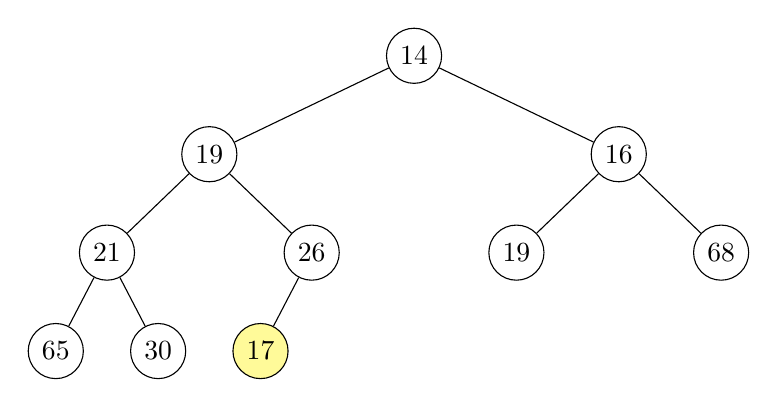
\begin{tikzpicture}[
  level distance=1.25cm,
  level 1/.style={sibling distance=5.2cm},
  level 2/.style={sibling distance=2.6cm},
  level 3/.style={sibling distance=1.3cm},
  level 4/.style={sibling distance=0.9cm},
  every node/.style={circle, draw, minimum size=7mm, inner sep=1pt},
  edge from parent/.style={draw,-}
]
\node {14}
  child { node {19}
    child { node {21}
      child { node {65} }
      child { node {30} }
    }
    child { node {26}
      child { node[fill=yellow!40] {17} }
      child[missing] {}
    }
  }
  child { node {16}
    child { node {19} }
    child { node {68} }
  };
\end{tikzpicture}
\end{center}

\textbf{Step 3: swap with parent 26 at index 5}

\[
[\text{EMPTY}, 14,19,16,21,17,19,68,65,30,26]
\]

\begin{center}
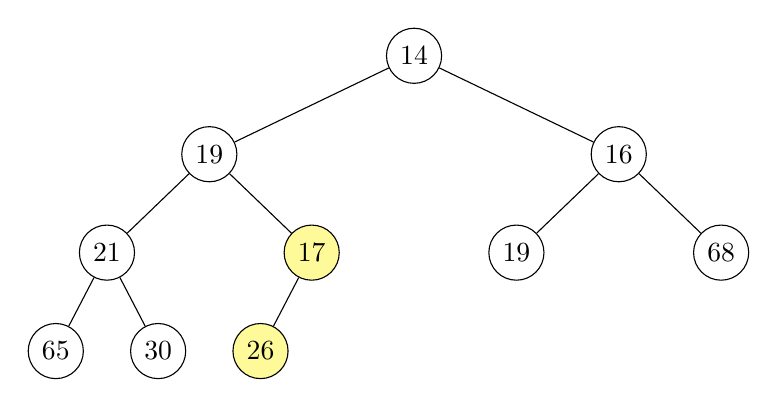
\begin{tikzpicture}[
  level distance=1.25cm,
  level 1/.style={sibling distance=5.2cm},
  level 2/.style={sibling distance=2.6cm},
  level 3/.style={sibling distance=1.3cm},
  level 4/.style={sibling distance=0.9cm},
  every node/.style={circle, draw, minimum size=7mm, inner sep=1pt},
  edge from parent/.style={draw,-}
]
\node {14}
  child { node {19}
    child { node {21}
      child { node {65} }
      child { node {30} }
    }
    child { node[fill=yellow!40] {17}
      child { node[fill=yellow!40] {26} }
      child[missing] {}
    }
  }
  child { node {16}
    child { node {19} }
    child { node {68} }
  };
\end{tikzpicture}
\end{center}

\textbf{Step 4: swap with parent 19 at index 2}

\[
[\text{EMPTY}, 14,17,16,21,19,19,68,65,30,26]
\]

\begin{center}
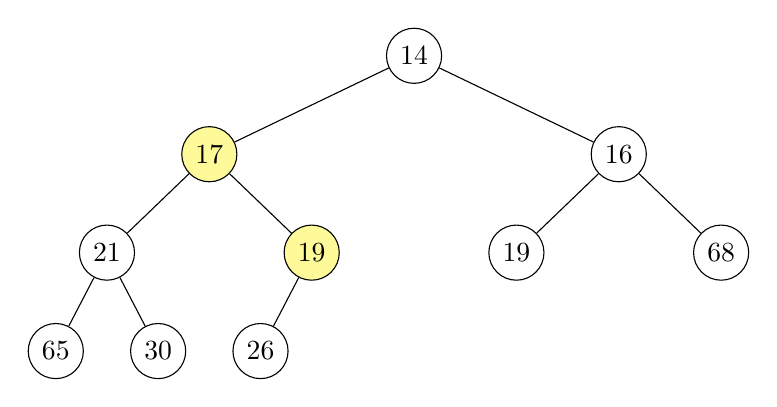
\begin{tikzpicture}[
  level distance=1.25cm,
  level 1/.style={sibling distance=5.2cm},
  level 2/.style={sibling distance=2.6cm},
  level 3/.style={sibling distance=1.3cm},
  level 4/.style={sibling distance=0.9cm},
  every node/.style={circle, draw, minimum size=7mm, inner sep=1pt},
  edge from parent/.style={draw,-}
]
\node {14}
  child { node[fill=yellow!40] {17}
    child { node {21}
      child { node {65} }
      child { node {30} }
    }
    child { node[fill=yellow!40] {19}
      child { node {26} }
      child[missing] {}
    }
  }
  child { node {16}
    child { node {19} }
    child { node {68} }
  };
\end{tikzpicture}
\end{center}

\textbf{Step 5: stop (Index 2 $>$ Index 1, $17 > 14$)}

Final heap:
\[
[\text{EMPTY}, 14,17,16,21,19,19,68,65,30,26]
\]
\textbf{Code:}
\begin{verbatim}
void push(int val) {
    heap.add(val);
    int i = heap.size() - 1;

    while (i > 1 && heap.get(i) < heap.get(i / 2)) {
        int temp = heap.get(i);
        heap.set(i, heap.get(i / 2));
        heap.set(i / 2, temp);
        i = i / 2;
    }
}
\end{verbatim}

\textbf{Time Complexity:} $O(\log n)$

\subsection{Pop (Remove Min)}

To pop from a min-heap:
\begin{itemize}
  \item Replace the root with the last element in the array
  \item Delete the last element
  \item Percolate down: Repeatedly swap the new root with its smaller child while it is larger, moving it downward until both children are larger than or equal to it.
\end{itemize}

\textbf{Step 1: Starting heap}

\[
[\text{EMPTY},\ 14,\ 19,\ 16,\ 21,\ 26,\ 19,\ 68,\ 65,\ 30]
\]

\begin{center}
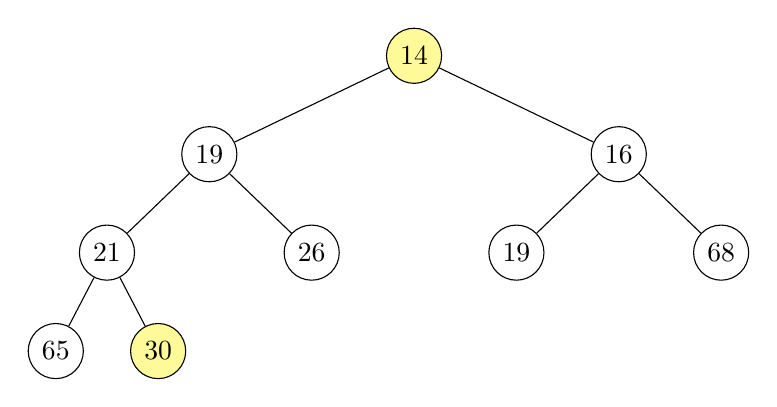
\begin{tikzpicture}[
  level distance=1.25cm,
  level 1/.style={sibling distance=5.2cm},
  level 2/.style={sibling distance=2.6cm},
  level 3/.style={sibling distance=1.3cm},
  every node/.style={circle, draw, minimum size=7mm, inner sep=1pt},
  edge from parent/.style={draw,-}
]
\node[fill=yellow!40] {14}
  child { node {19}
    child { node {21}
      child { node {65} }
      child { node[fill=yellow!40] {30} }
    }
    child { node {26} }
  }
  child { node {16}
    child { node {19} }
    child { node {68} }
  };
\end{tikzpicture}
\end{center}

\textbf{Step 2: swap root with last (30), delete the original root}

\[
[\text{EMPTY}, 30,19,16,21,26,19,68,65]
\]

\begin{center}
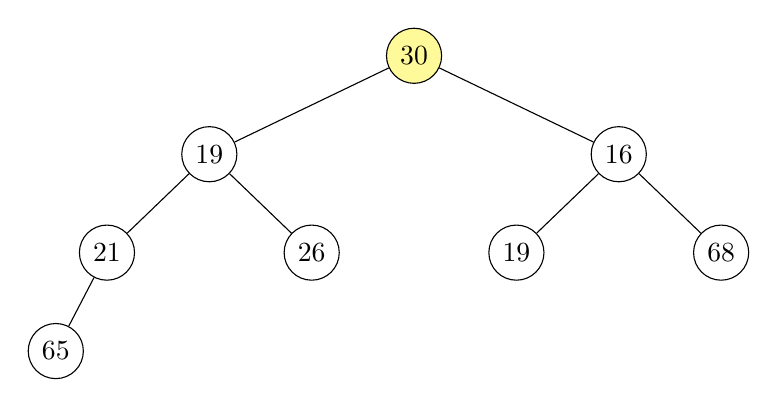
\begin{tikzpicture}[
  level distance=1.25cm,
  level 1/.style={sibling distance=5.2cm},
  level 2/.style={sibling distance=2.6cm},
  level 3/.style={sibling distance=1.3cm},
  every node/.style={circle, draw, minimum size=7mm, inner sep=1pt},
  edge from parent/.style={draw,-}
]
\node[fill=yellow!40] {30}
  child { node {19}
    child { node {21}
      child { node {65} }
      child[missing] {}
    }
    child { node {26} }
  }
  child { node {16}
    child { node {19} }
    child { node {68} }
  };
\end{tikzpicture}
\end{center}

\textbf{Step 3: percolate down, swapping with the smaller child (16)}

\[
[\text{EMPTY}, 16,19,30,21,26,19,68,65]
\]

\begin{center}
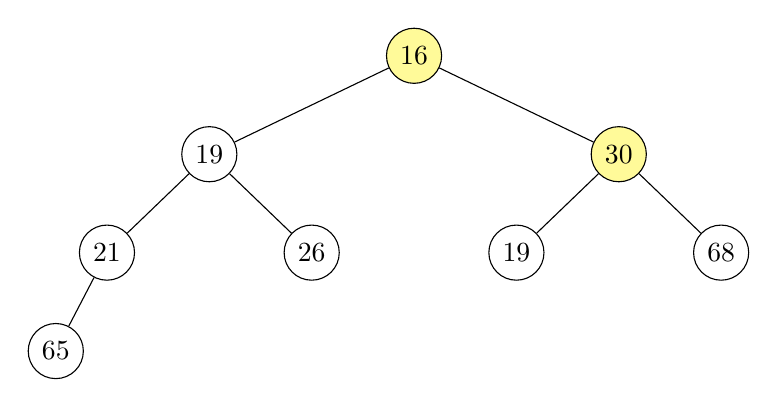
\begin{tikzpicture}[
  level distance=1.25cm,
  level 1/.style={sibling distance=5.2cm},
  level 2/.style={sibling distance=2.6cm},
  level 3/.style={sibling distance=1.3cm},
  every node/.style={circle, draw, minimum size=7mm, inner sep=1pt},
  edge from parent/.style={draw,-}
]
\node[fill=yellow!40] {16}
  child { node {19}
    child { node {21}
      child { node {65} }
      child[missing] {}
    }
    child { node {26} }
  }
  child { node[fill=yellow!40] {30}
    child { node {19} }
    child { node {68} }
  };
\end{tikzpicture}
\end{center}

\textbf{Step 4: swap with smaller child (19)}

\[
[\text{EMPTY}, 16,19,19,21,26,30,68,65]
\]

\begin{center}
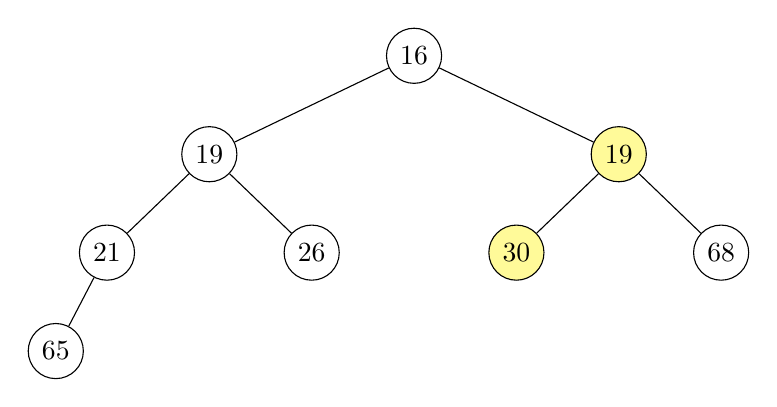
\begin{tikzpicture}[
  level distance=1.25cm,
  level 1/.style={sibling distance=5.2cm},
  level 2/.style={sibling distance=2.6cm},
  level 3/.style={sibling distance=1.3cm},
  every node/.style={circle, draw, minimum size=7mm, inner sep=1pt},
  edge from parent/.style={draw,-}
]
\node {16}
  child { node {19}
    child { node {21}
      child { node {65} }
      child[missing] {}
    }
    child { node {26} }
  }
  child { node[fill=yellow!40] {19}
    child { node[fill=yellow!40] {30} }
    child { node {68} }
  };
\end{tikzpicture}
\end{center}

Final heap:
\[
[\text{EMPTY}, 16,19,19,21,26,30,68,65]
\]
\textbf{Code:}
\begin{verbatim}
int pop() {
    int res = heap.get(1);
    heap.set(1, heap.get(heap.size() - 1));
    heap.remove(heap.size() - 1);

    int i = 1;
    while (2 * i < heap.size()) {
        int smallest = 2 * i;
        if (2 * i + 1 < heap.size()
                && heap.get(2 * i + 1) < heap.get(2 * i))
            smallest = 2 * i + 1;

        if (heap.get(i) > heap.get(smallest)) {
            int temp = heap.get(i);
            heap.set(i, heap.get(smallest));
            heap.set(smallest, temp);
            i = smallest;
        } else break;
    }
    return res;
}
\end{verbatim}

\textbf{Time Complexity:} $O(\log n)$

\subsection{Heapify (Build Heap in $O(n)$)}
Heapify builds a heap from an unsorted array more efficiently than repeated inserts.

\textbf{Step 1: Starting array (unsorted)}
\[
[\text{EMPTY}, 50,80,40,30,10,70,20,90,60]
\]
\begin{center}
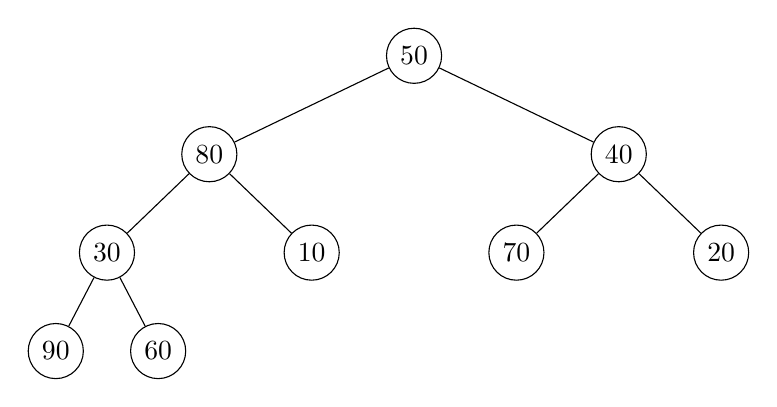
\begin{tikzpicture}[
  level distance=1.25cm,
  level 1/.style={sibling distance=5.2cm},
  level 2/.style={sibling distance=2.6cm},
  level 3/.style={sibling distance=1.3cm},
  every node/.style={circle, draw, minimum size=7mm, inner sep=1pt},
  edge from parent/.style={draw,-}
]
\node {50}
  child { node {80}
    child { node {30}
      child { node {90} }
      child { node {60} }
    }
    child { node {10} }
  }
  child { node {40}
    child { node {70} }
    child { node {20} }
  };
\end{tikzpicture}
\end{center}
Heapify starts at $i = \lfloor n/2 \rfloor = 4$ (node 30), the last node with children (left child = $2i$), and percolates down to the root.

\textbf{Step 2: Process node at index 4 (value 30)}

30 has children 90 and 60. Since $30 < 60$ and $30 < 90$, no swap needed.
\[
[\text{EMPTY}, 50,80,40,30,10,70,20,90,60]
\]
\begin{center}
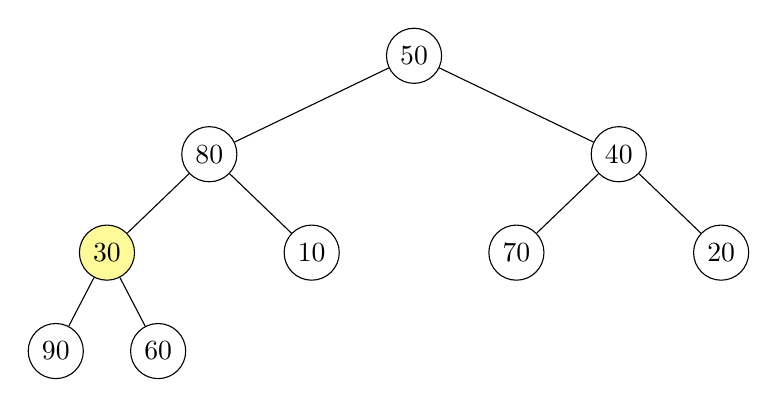
\begin{tikzpicture}[
  level distance=1.25cm,
  level 1/.style={sibling distance=5.2cm},
  level 2/.style={sibling distance=2.6cm},
  level 3/.style={sibling distance=1.3cm},
  every node/.style={circle, draw, minimum size=7mm, inner sep=1pt},
  edge from parent/.style={draw,-}
]
\node {50}
  child { node {80}
    child { node[fill=yellow!40] {30}
      child { node {90} }
      child { node {60} }
    }
    child { node {10} }
  }
  child { node {40}
    child { node {70} }
    child { node {20} }
  };
\end{tikzpicture}
\end{center}

\textbf{Step 3: Process node at index 3 (value 40)}

40 has children 70 and 20. Smaller child is 20. Since $40 > 20$, swap 40 and 20.
\[
[\text{EMPTY}, 50,80,20,30,10,70,40,90,60]
\]
\begin{center}
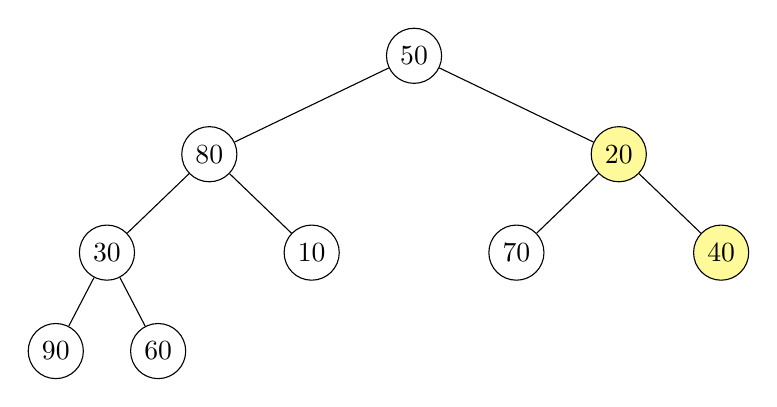
\begin{tikzpicture}[
  level distance=1.25cm,
  level 1/.style={sibling distance=5.2cm},
  level 2/.style={sibling distance=2.6cm},
  level 3/.style={sibling distance=1.3cm},
  every node/.style={circle, draw, minimum size=7mm, inner sep=1pt},
  edge from parent/.style={draw,-}
]
\node {50}
  child { node {80}
    child { node {30}
      child { node {90} }
      child { node {60} }
    }
    child { node {10} }
  }
  child { node[fill=yellow!40] {20}
    child { node {70} }
    child { node[fill=yellow!40] {40} }
  };
\end{tikzpicture}
\end{center}

40 has no children, so we can stop percolating down.

\textbf{Step 4: Process node at index 2 (value 80)}

80 has children 30 and 10. Smaller child is 10. Since $80 > 10$, swap 80 and 10.
\[
[\text{EMPTY},50,10,20,30,80,70,40,90,60]
\]
\begin{center}
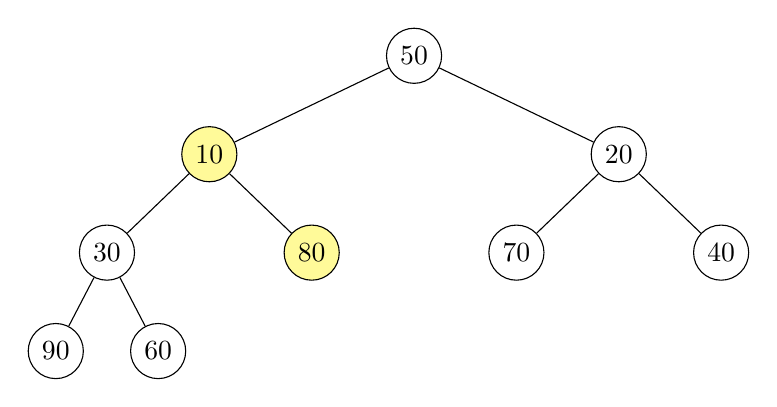
\begin{tikzpicture}[
  level distance=1.25cm,
  level 1/.style={sibling distance=5.2cm},
  level 2/.style={sibling distance=2.6cm},
  level 3/.style={sibling distance=1.3cm},
  every node/.style={circle, draw, minimum size=7mm, inner sep=1pt},
  edge from parent/.style={draw,-}
]
\node {50}
  child { node[fill=yellow!40] {10}
    child { node {30}
      child { node {90} }
      child { node {60} }
    }
    child { node[fill=yellow!40] {80} }
  }
  child { node {20}
    child { node {70} }
    child { node {40} }
  };
\end{tikzpicture}
\end{center}

80 has no children, so we can stop percolating down.

\textbf{Step 5: Process node at index 1 (value 50, the root)}

50 has children 10 and 20. Smaller child is 10. Since $50 > 10$, swap 50 and 10.
\[
[\text{EMPTY},10,50,20,30,80,70,40,90,60]
\]
\begin{center}
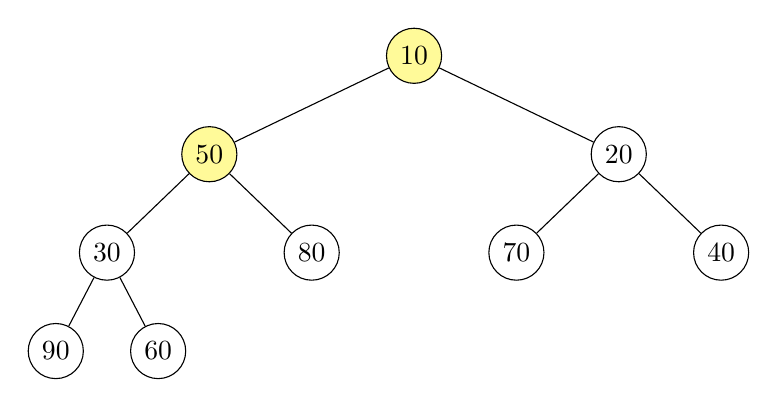
\begin{tikzpicture}[
  level distance=1.25cm,
  level 1/.style={sibling distance=5.2cm},
  level 2/.style={sibling distance=2.6cm},
  level 3/.style={sibling distance=1.3cm},
  every node/.style={circle, draw, minimum size=7mm, inner sep=1pt},
  edge from parent/.style={draw,-}
]
\node[fill=yellow!40] {10}
  child { node[fill=yellow!40] {50}
    child { node {30}
      child { node {90} }
      child { node {60} }
    }
    child { node {80} }
  }
  child { node {20}
    child { node {70} }
    child { node {40} }
  };
\end{tikzpicture}
\end{center}

\textbf{Step 6: Continue percolating the original root down}

50 has children 30 and 80. Smaller child is 30. Since $50 > 30$, swap 50 and 30.
\[
[10,30,20,50,80,70,40,90,60]
\]
\begin{center}
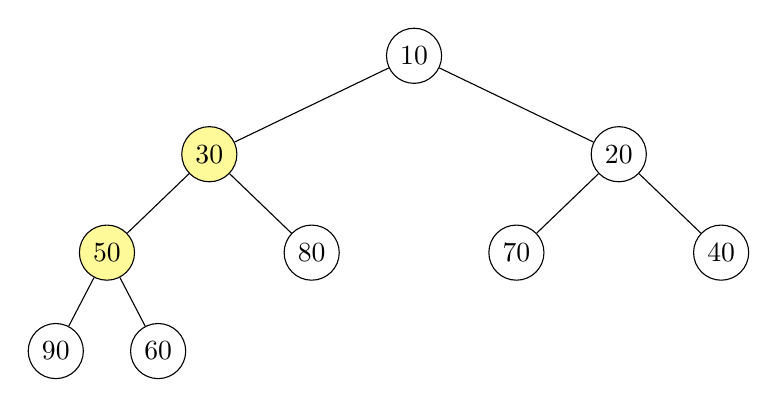
\begin{tikzpicture}[
  level distance=1.25cm,
  level 1/.style={sibling distance=5.2cm},
  level 2/.style={sibling distance=2.6cm},
  level 3/.style={sibling distance=1.3cm},
  every node/.style={circle, draw, minimum size=7mm, inner sep=1pt},
  edge from parent/.style={draw,-}
]
\node {10}
  child { node[fill=yellow!40] {30}
    child { node[fill=yellow!40] {50}
      child { node {90} }
      child { node {60} }
    }
    child { node {80} }
  }
  child { node {20}
    child { node {70} }
    child { node {40} }
  };
\end{tikzpicture}
\end{center}

\textbf{Step 7: Continue percolating 50 down}

50 has children 90 and 60. Smaller child is 60. Since $50 < 60$, stop. Heap property satisfied.

\textbf{Final heap:}
\[
[10,30,20,50,80,70,40,90,60]
\]
\begin{center}
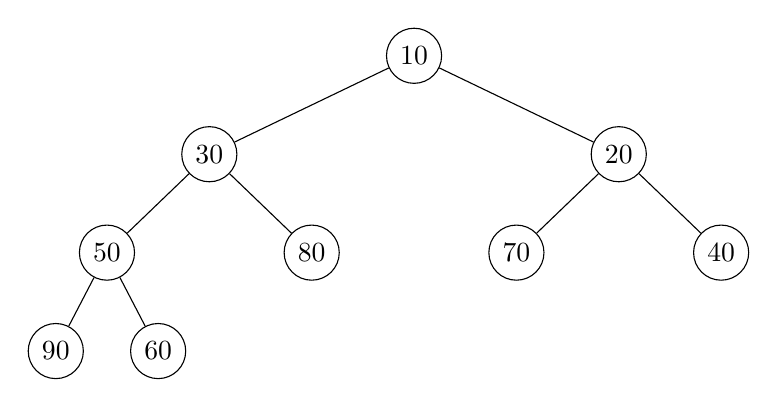
\begin{tikzpicture}[
  level distance=1.25cm,
  level 1/.style={sibling distance=5.2cm},
  level 2/.style={sibling distance=2.6cm},
  level 3/.style={sibling distance=1.3cm},
  every node/.style={circle, draw, minimum size=7mm, inner sep=1pt},
  edge from parent/.style={draw,-}
]
\node {10}
  child { node {30}
    child { node {50}
      child { node {90} }
      child { node {60} }
    }
    child { node {80} }
  }
  child { node {20}
    child { node {70} }
    child { node {40} }
  };
\end{tikzpicture}
\end{center}
\textbf{Code:}
\begin{verbatim}
void heapify(List<Integer> a) {
    a.add(0, 0); // dummy for 1-based indexing
    for (int i = (a.size() - 1) / 2; i >= 1; i--) {
        int j = i;
        while (2 * j < a.size()) {
            int c = 2 * j;
            if (c + 1 < a.size() && a.get(c + 1) < a.get(c))
                c++;
            if (a.get(j) > a.get(c)) {
                int temp = a.get(j);
                a.set(j, a.get(c));
                a.set(c, temp);
                j = c;
            } else break;
        }
    }
}
\end{verbatim}

Heapify is $O(n)$ because most nodes are near the bottom and percolate down only a few levels, while the few nodes near the top that percolate far down are outnumbered.

\subsection{Time Complexities}
\begin{center}
\begin{tabular}{l c}
\toprule
Operation & Time \\
\midrule
Get Min / Max & $O(1)$ \\
Push & $O(\log n)$ \\
Pop & $O(\log n)$ \\
Heapify & $O(n)$ \\
\bottomrule
\end{tabular}
\end{center}
\section{Graphs}

A \textbf{graph} is a data structure made up of \textbf{nodes} connected by \textbf{pointers}.
Graphs are used to model relationships between entities, such as:
\begin{itemize}
  \item Social networks (one person follows another)
  \item Maps (one city connected to another)
  \item Dependencies (one task must be completed before another)
\end{itemize}

\subsection{Graph Terminology}

In graphs:
\begin{itemize}
  \item Nodes are called \textbf{vertices}
  \item Pointers connecting nodes are called \textbf{edges}
\end{itemize}

Unlike trees and linked lists, graphs have \textbf{no restrictions} on how nodes are connected:
\begin{itemize}
  \item A node can have any number of edges
  \item Cycles are allowed
  \item Nodes don't need to be connected at all
\end{itemize}

The only restriction is the maximum number of edges:
\[
E \leq V^2
\]
This is because every vertex can have an edge pointed to every other vertex \textbf{plus itself}, leading to a maximum of $V^2$ edges. A graph with $V$ vertices and $V^2$ edges is called a \textbf{complete graph}.

\subsection{Directed vs Undirected Graphs}

\textbf{Directed Graph:}
Edges have a direction. An edge from $A$ to $B$ does \textbf{not} imply an edge from $B$ to $A$.

\begin{center}
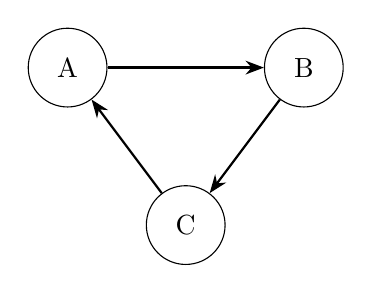
\begin{tikzpicture}[
  >=Stealth,
  every node/.style={circle, draw, minimum size=10mm},
  edge/.style={->, thick}
]
\node (A) at (0,0) {A};
\node (B) at (3,0) {B};
\node (C) at (1.5,-2) {C};

\draw[edge] (A) -- (B);
\draw[edge] (B) -- (C);
\draw[edge] (C) -- (A);
\end{tikzpicture}

{\small Directed graph: $C \to A$ exists, but $A \to C$ does not}
\end{center}

Trees and linked lists are examples of directed graphs (pointers like \texttt{prev}, \texttt{next}, \texttt{left}, \texttt{right}).

\textbf{Undirected Graph:}
Edges have no direction. If there's an edge between $A$ and $B$, you can traverse in both directions.

\begin{center}
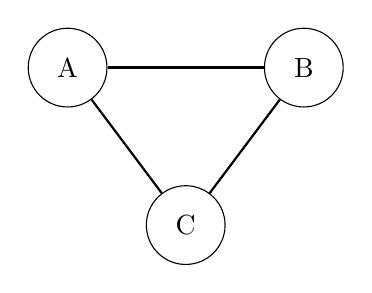
\begin{tikzpicture}[
  every node/.style={circle, draw, minimum size=10mm},
  edge/.style={-, thick}
]
\node (A) at (0,0) {A};
\node (B) at (3,0) {B};
\node (C) at (1.5,-2) {C};

\draw[edge] (A) -- (B);
\draw[edge] (B) -- (C);
\draw[edge] (C) -- (A);
\end{tikzpicture}

{\small Undirected graph: can traverse A--C in both directions}
\end{center}

\subsection{Matrix (Grid)}

Graphs can be represented using different data structures. The first representation is a Matrix.

A \textbf{matrix} is a 2D array where:
\begin{itemize}
  \item \texttt{0} represents a free cell (vertex)
  \item \texttt{1} represents a blocked cell
\end{itemize}

\begin{verbatim}
int[][] grid = {{0, 0, 0, 0},
                {1, 1, 0, 0},
                {0, 0, 0, 1},
                {0, 1, 0, 0}};
\end{verbatim}

To traverse the graph, we move \textbf{up, down, left, right} between adjacent 0s. Connected 0s form \textbf{connected components}.

\begin{center}
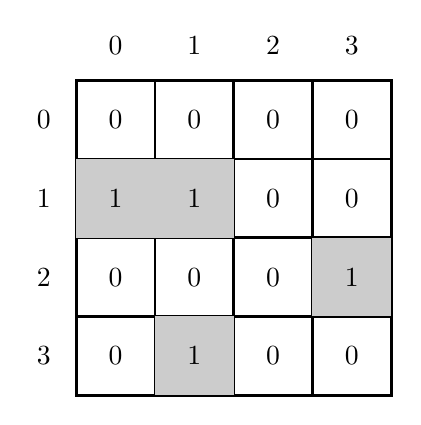
\begin{tikzpicture}[x=1cm,y=1cm]
  \def\cellW{1.0}
  \def\H{1.0}
  
  % Draw grid
  \foreach \row in {0,...,3} {
    \foreach \col in {0,...,3} {
      \draw[line width=1pt] ({\col*\cellW},{-\row*\H}) rectangle ({(\col+1)*\cellW},{(-\row-1)*\H});
    }
  }
  
  % Fill blocked cells (1s)
  \fill[gray!40] ({0*\cellW},{-1*\H}) rectangle ({1*\cellW},{-2*\H}); % [1][0]
  \fill[gray!40] ({1*\cellW},{-1*\H}) rectangle ({2*\cellW},{-2*\H}); % [1][1]
  \fill[gray!40] ({3*\cellW},{-2*\H}) rectangle ({4*\cellW},{-3*\H}); % [2][3]
  \fill[gray!40] ({1*\cellW},{-3*\H}) rectangle ({2*\cellW},{-4*\H}); % [3][1]
  
  % Add values
  \node at ({0.5*\cellW},{-0.5*\H}) {0};
  \node at ({1.5*\cellW},{-0.5*\H}) {0};
  \node at ({2.5*\cellW},{-0.5*\H}) {0};
  \node at ({3.5*\cellW},{-0.5*\H}) {0};
  
  \node at ({0.5*\cellW},{-1.5*\H}) {1};
  \node at ({1.5*\cellW},{-1.5*\H}) {1};
  \node at ({2.5*\cellW},{-1.5*\H}) {0};
  \node at ({3.5*\cellW},{-1.5*\H}) {0};
  
  \node at ({0.5*\cellW},{-2.5*\H}) {0};
  \node at ({1.5*\cellW},{-2.5*\H}) {0};
  \node at ({2.5*\cellW},{-2.5*\H}) {0};
  \node at ({3.5*\cellW},{-2.5*\H}) {1};
  
  \node at ({0.5*\cellW},{-3.5*\H}) {0};
  \node at ({1.5*\cellW},{-3.5*\H}) {1};
  \node at ({2.5*\cellW},{-3.5*\H}) {0};
  \node at ({3.5*\cellW},{-3.5*\H}) {0};
  
  % Row/column labels
  \node[anchor=east] at (-0.2,-0.5) {0};
  \node[anchor=east] at (-0.2,-1.5) {1};
  \node[anchor=east] at (-0.2,-2.5) {2};
  \node[anchor=east] at (-0.2,-3.5) {3};
  
  \node[anchor=south] at (0.5,0.2) {0};
  \node[anchor=south] at (1.5,0.2) {1};
  \node[anchor=south] at (2.5,0.2) {2};
  \node[anchor=south] at (3.5,0.2) {3};
\end{tikzpicture}
\end{center}

\textbf{Space Complexity:} $O(n \cdot m)$ where $n$ is rows and $m$ is columns.

\subsection{Adjacency Matrix}

An \textbf{adjacency matrix} is another representation, and is a 2D array where indices represent vertices:
\begin{itemize}
  \item \texttt{adjMatrix[v1][v2] = 1} means an edge exists from \texttt{v1} to \texttt{v2}
  \item \texttt{adjMatrix[v1][v2] = 0} means no edge exists from \texttt{v1} to \texttt{v2}
\end{itemize}

\begin{verbatim}
int[][] adjMatrix = {{0, 0, 0, 0},
                     {1, 1, 0, 0},
                     {0, 0, 0, 1},
                     {0, 1, 0, 0}};
\end{verbatim}

\begin{center}
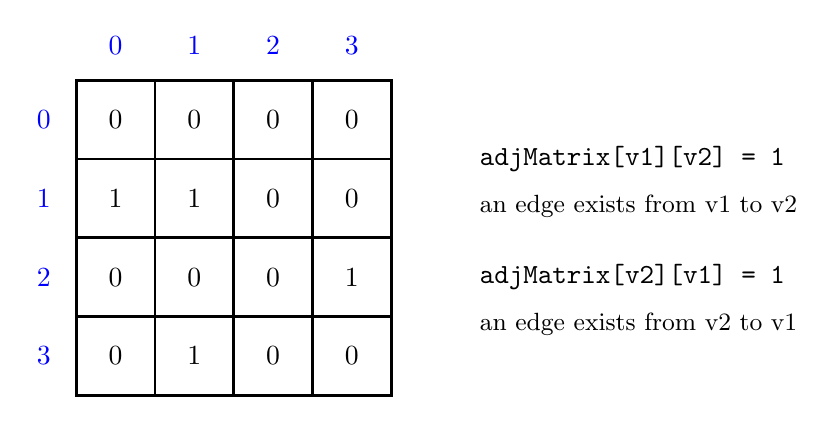
\begin{tikzpicture}[x=1cm,y=1cm]
  \def\cellW{1.0}
  \def\H{1.0}
  
  % Draw grid
  \foreach \row in {0,...,3} {
    \foreach \col in {0,...,3} {
      \draw[line width=1pt] ({\col*\cellW},{-\row*\H}) rectangle ({(\col+1)*\cellW},{(-\row-1)*\H});
    }
  }
  
  % Add values - row 0
  \node at ({0.5*\cellW},{-0.5*\H}) {0};
  \node at ({1.5*\cellW},{-0.5*\H}) {0};
  \node at ({2.5*\cellW},{-0.5*\H}) {0};
  \node at ({3.5*\cellW},{-0.5*\H}) {0};
  
  % Row 1
  \node at ({0.5*\cellW},{-1.5*\H}) {1};
  \node at ({1.5*\cellW},{-1.5*\H}) {1};
  \node at ({2.5*\cellW},{-1.5*\H}) {0};
  \node at ({3.5*\cellW},{-1.5*\H}) {0};
  
  % Row 2
  \node at ({0.5*\cellW},{-2.5*\H}) {0};
  \node at ({1.5*\cellW},{-2.5*\H}) {0};
  \node at ({2.5*\cellW},{-2.5*\H}) {0};
  \node at ({3.5*\cellW},{-2.5*\H}) {1};
  
  % Row 3
  \node at ({0.5*\cellW},{-3.5*\H}) {0};
  \node at ({1.5*\cellW},{-3.5*\H}) {1};
  \node at ({2.5*\cellW},{-3.5*\H}) {0};
  \node at ({3.5*\cellW},{-3.5*\H}) {0};
  
  % Row/column labels
  \node[anchor=east,blue] at (-0.2,-0.5) {0};
  \node[anchor=east,blue] at (-0.2,-1.5) {1};
  \node[anchor=east,blue] at (-0.2,-2.5) {2};
  \node[anchor=east,blue] at (-0.2,-3.5) {3};
  
  \node[anchor=south,blue] at (0.5,0.2) {0};
  \node[anchor=south,blue] at (1.5,0.2) {1};
  \node[anchor=south,blue] at (2.5,0.2) {2};
  \node[anchor=south,blue] at (3.5,0.2) {3};
  
  % Annotations
  \node[anchor=west] at (5,-1) {\texttt{adjMatrix[v1][v2] = 1}};
  \node[anchor=west] at (5,-1.6) {\small an edge exists from v1 to v2};
  
  \node[anchor=west] at (5,-2.5) {\texttt{adjMatrix[v2][v1] = 1}};
  \node[anchor=west] at (5,-3.1) {\small an edge exists from v2 to v1};
\end{tikzpicture}
\end{center}

From the matrix above:
\begin{itemize}
  \item \texttt{adjMatrix[1][0] = 1}: edge from vertex 1 to vertex 0
  \item \texttt{adjMatrix[1][1] = 1}: edge from vertex 1 to itself (self-loop)
  \item \texttt{adjMatrix[2][3] = 1}: edge from vertex 2 to vertex 3
  \item \texttt{adjMatrix[3][1] = 1}: edge from vertex 3 to vertex 1
\end{itemize}

\begin{center}
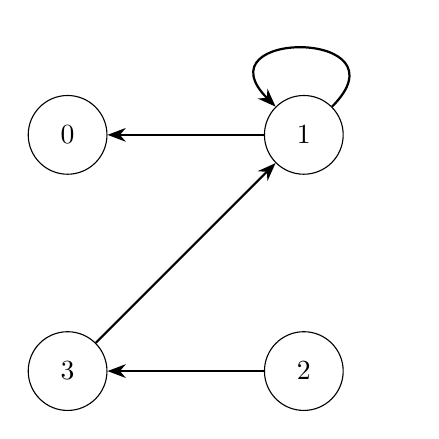
\begin{tikzpicture}[
  >=Stealth,
  every node/.style={circle, draw, minimum size=10mm},
  edge/.style={->, thick}
]
\node (0) at (0,0) {0};
\node (1) at (3,0) {1};
\node (2) at (3,-3) {2};
\node (3) at (0,-3) {3};

\draw[edge] (1) -- (0);
\draw[edge] (1) to [out=45,in=135,looseness=5] (1); % self-loop
\draw[edge] (2) -- (3);
\draw[edge] (3) -- (1);
\end{tikzpicture}

{\small Graph represented by the adjacency matrix}
\end{center}

\textbf{Drawback:} If the graph has few edges, most of the matrix is wasted storing 0s.

\textbf{Space Complexity:} $O(V^2)$ where $V$ is the number of vertices.

\subsection{Adjacency List}

Another common way to represent a graph is with an \textbf{adjacency list}, where each vertex maps to a list of its neighboring vertices. An adjacency list is more efficiently stored as a \textbf{List} or  \textbf{HashMap}, where each key is a vertex and the value is the list of its neighbors, allowing $O(1)$ average-time lookups. For example, given the following directed graph:

\begin{center}
\begin{tikzpicture}[
  >=Stealth,
  every node/.style={circle, draw, minimum size=10mm},
  edge/.style={->, thick}
]
\node (A) at (0,0) {A};
\node (B) at (0,-2) {B};
\node (C) at (0,-4) {C};
\node (D) at (3,0) {D};
\node (E) at (3,-2.5) {E};

\draw[edge] (A) -- (B);
\draw[edge] (B) -- (C);
\draw[edge] (B) -- (E);
\draw[edge] (C) -- (E);
\draw[edge] (E) -- (D);
\end{tikzpicture}
\end{center}
The adjacency list equivalent is:

\begin{center}
\begin{tikzpicture}[x=1cm,y=1cm,>=Stealth]
  % Node boxes
  \foreach \i/\val in {0/A, 1/B, 2/C, 3/D, 4/E} {
    % Node value box
    \draw[line width=1pt] (0,{-\i*1.2}) rectangle (1,{-\i*1.2-0.8});
    \node at (0.5,{-\i*1.2-0.4}) {\val};
    
    % Arrow to neighbors
    \draw[->,thick] (1,{-\i*1.2-0.4}) -- (1.5,{-\i*1.2-0.4});
  }
  
  % Neighbor lists
  \node[anchor=west] at (1.6,-0.4) {[B]};
  \node[anchor=west] at (1.6,-1.6) {[C, E]};
  \node[anchor=west] at (1.6,-2.8) {[E]};
  \node[anchor=west] at (1.6,-4.0) {[ ]};
  \node[anchor=west] at (1.6,-5.2) {[D]};
  
  % Labels
  \node[anchor=east] at (-0.2,-0.4) {vertex A:};
  \node[anchor=east] at (-0.2,-1.6) {vertex B:};
  \node[anchor=east] at (-0.2,-2.8) {vertex C:};
  \node[anchor=east] at (-0.2,-4.0) {vertex D:};
  \node[anchor=east] at (-0.2,-5.2) {vertex E:};
\end{tikzpicture}
\end{center}

\subsubsection{DFS (contains a path)}

We can traverse an adjacency list using \textbf{Depth-First Search (DFS)}. The algorithm marks each vertex as visited and records the edge used to reach it, allowing us to reconstruct the path from any vertex back to the source.

\textbf{Example: DFS from A (source = A)}

\textbf{Step 1:} Mark A as visited. Check neighbors: B is unmarked, set \texttt{edgeTo[B] = A}. Visit B.

\begin{center}
\begin{tikzpicture}[
  >=Stealth,
  every node/.style={circle, draw, minimum size=10mm},
  edge/.style={->, thick},
  highlight/.style={circle, draw, fill=blue!20, minimum size=10mm},
  hedge/.style={->, thick, blue}
]
\node[highlight] (A) at (0,0) {A};
\node (B) at (0,-2) {B};
\node (C) at (0,-4) {C};
\node (D) at (3,0) {D};
\node (E) at (3,-2.5) {E};

\draw[hedge] (A) -- (B);
\draw[edge] (B) -- (C);
\draw[edge] (B) -- (E);
\draw[edge] (C) -- (E);
\draw[edge] (E) -- (D);
\end{tikzpicture}

{\small marked = \{A\} \quad edgeTo[B] = A}
\end{center}

\textbf{Step 2:} Mark B as visited. Check neighbors: C is unmarked, set \texttt{edgeTo[C] = B}. Visit C.

\begin{center}
\begin{tikzpicture}[
  >=Stealth,
  every node/.style={circle, draw, minimum size=10mm},
  edge/.style={->, thick},
  highlight/.style={circle, draw, fill=blue!20, minimum size=10mm},
  hedge/.style={->, thick, blue}
]
\node[highlight] (A) at (0,0) {A};
\node[highlight] (B) at (0,-2) {B};
\node (C) at (0,-4) {C};
\node (D) at (3,0) {D};
\node (E) at (3,-2.5) {E};

\draw[hedge] (A) -- (B);
\draw[hedge] (B) -- (C);
\draw[edge] (B) -- (E);
\draw[edge] (C) -- (E);
\draw[edge] (E) -- (D);
\end{tikzpicture}

{\small marked = \{A, B\} \quad edgeTo[C] = B}
\end{center}

\textbf{Step 3:} Mark C as visited. Check neighbors: E is unmarked, set \texttt{edgeTo[E] = C}. Visit E.

\begin{center}
\begin{tikzpicture}[
  >=Stealth,
  every node/.style={circle, draw, minimum size=10mm},
  edge/.style={->, thick},
  highlight/.style={circle, draw, fill=blue!20, minimum size=10mm},
  hedge/.style={->, thick, blue}
]
\node[highlight] (A) at (0,0) {A};
\node[highlight] (B) at (0,-2) {B};
\node[highlight] (C) at (0,-4) {C};
\node (D) at (3,0) {D};
\node (E) at (3,-2.5) {E};

\draw[hedge] (A) -- (B);
\draw[hedge] (B) -- (C);
\draw[edge] (B) -- (E);
\draw[hedge] (C) -- (E);
\draw[edge] (E) -- (D);
\end{tikzpicture}

{\small marked = \{A, B, C\} \quad edgeTo[E] = C}
\end{center}

\textbf{Step 4:} Mark E as visited. Check neighbors: D is unmarked, set \texttt{edgeTo[D] = E}. Visit D.

\begin{center}
\begin{tikzpicture}[
  >=Stealth,
  every node/.style={circle, draw, minimum size=10mm},
  edge/.style={->, thick},
  highlight/.style={circle, draw, fill=blue!20, minimum size=10mm},
  hedge/.style={->, thick, blue}
]
\node[highlight] (A) at (0,0) {A};
\node[highlight] (B) at (0,-2) {B};
\node[highlight] (C) at (0,-4) {C};
\node (D) at (3,0) {D};
\node[highlight] (E) at (3,-2.5) {E};

\draw[hedge] (A) -- (B);
\draw[hedge] (B) -- (C);
\draw[edge] (B) -- (E);
\draw[hedge] (C) -- (E);
\draw[hedge] (E) -- (D);
\end{tikzpicture}

{\small marked = \{A, B, C, E\} \quad edgeTo[D] = E}
\end{center}

\textbf{Step 5:} Mark D as visited. D has no unmarked neighbors. Backtrack to E, then B. B's second neighbor E is already marked. Done.

\begin{center}
\begin{tikzpicture}[
  >=Stealth,
  every node/.style={circle, draw, minimum size=10mm},
  edge/.style={->, thick},
  highlight/.style={circle, draw, fill=blue!20, minimum size=10mm},
  hedge/.style={->, thick, blue}
]
\node[highlight] (A) at (0,0) {A};
\node[highlight] (B) at (0,-2) {B};
\node[highlight] (C) at (0,-4) {C};
\node[highlight] (D) at (3,0) {D};
\node[highlight] (E) at (3,-2.5) {E};

\draw[hedge] (A) -- (B);
\draw[hedge] (B) -- (C);
\draw[edge] (B) -- (E);
\draw[hedge] (C) -- (E);
\draw[hedge] (E) -- (D);
\end{tikzpicture}

{\small All vertices marked.}
\end{center}

Using \texttt{edgeTo}, we can reconstruct the path from A to any vertex. For example, the path from A to D: follow \texttt{edgeTo[D] = E}, \texttt{edgeTo[E] = C}, \texttt{edgeTo[C] = B}, \texttt{edgeTo[B] = A}, giving us $A \rightarrow B \rightarrow C \rightarrow E \rightarrow D$.

To implement this, we use the following code:
\begin{verbatim}
public class DepthFirstPaths {
    Set<String> marked;
    Map<String, String> edgeTo;
    String s;

    public DepthFirstPaths(Graph G, String s) {
        marked = new HashSet<>();
        edgeTo = new HashMap<>();
        this.s = s;
        dfs(G, s);
    }

    private void dfs(Graph G, String v) {
        marked.add(v);
        for (String w : G.adj(v)) {
            if (!marked.contains(w)) {
                edgeTo.put(w, v);
                dfs(G, w);
            }
        }
    }
}
\end{verbatim}


\textbf{Time Complexity:} The time complexity for this DFS algorithm is
\[
O(V + E),
\]
as each vertex is visited once, and each edge is checked once for unvisited vertices.


\begin{itemize}
  \item \texttt{marked[v]}: whether vertex \texttt{v} has been visited
  \item \texttt{edgeTo[w] = v}: vertex \texttt{v} was used to reach \texttt{w}
  \item \texttt{G.adj(v)}: the adjacency list of vertex \texttt{v}
\end{itemize}

\subsubsection{DFS: number of unique paths}
We can use DFS to find the total number of unique paths to a targe node. 

\textbf{Example: count all unique paths from A to E}

\textbf{Step 1:} Start at A. A $\neq$ E, add A to visited. Visit neighbor B.

\begin{center}
\begin{tikzpicture}[
  >=Stealth,
  every node/.style={circle, draw, minimum size=10mm},
  edge/.style={->, thick},
  highlight/.style={circle, draw, fill=blue!20, minimum size=10mm},
  hedge/.style={->, thick, blue}
]
\node[highlight] (A) at (0,0) {A};
\node (B) at (0,-2) {B};
\node (C) at (0,-4) {C};
\node (D) at (3,0) {D};
\node (E) at (3,-2.5) {E};

\draw[hedge] (A) -- (B);
\draw[edge] (B) -- (C);
\draw[edge] (B) -- (E);
\draw[edge] (C) -- (E);
\draw[edge] (E) -- (D);
\end{tikzpicture}

{\small visited = \{A\}}
\end{center}

\textbf{Step 2:} At B. B $\neq$ E, add B to visited. Visit first neighbor C.

\begin{center}
\begin{tikzpicture}[
  >=Stealth,
  every node/.style={circle, draw, minimum size=10mm},
  edge/.style={->, thick},
  highlight/.style={circle, draw, fill=blue!20, minimum size=10mm},
  hedge/.style={->, thick, blue}
]
\node[highlight] (A) at (0,0) {A};
\node[highlight] (B) at (0,-2) {B};
\node (C) at (0,-4) {C};
\node (D) at (3,0) {D};
\node (E) at (3,-2.5) {E};

\draw[hedge] (A) -- (B);
\draw[hedge] (B) -- (C);
\draw[edge] (B) -- (E);
\draw[edge] (C) -- (E);
\draw[edge] (E) -- (D);
\end{tikzpicture}

{\small visited = \{A, B\}}
\end{center}

\textbf{Step 3:} At C. C $\neq$ E, add C to visited. Visit neighbor E.

\begin{center}
\begin{tikzpicture}[
  >=Stealth,
  every node/.style={circle, draw, minimum size=10mm},
  edge/.style={->, thick},
  highlight/.style={circle, draw, fill=blue!20, minimum size=10mm},
  hedge/.style={->, thick, blue}
]
\node[highlight] (A) at (0,0) {A};
\node[highlight] (B) at (0,-2) {B};
\node[highlight] (C) at (0,-4) {C};
\node (D) at (3,0) {D};
\node (E) at (3,-2.5) {E};

\draw[hedge] (A) -- (B);
\draw[hedge] (B) -- (C);
\draw[edge] (B) -- (E);
\draw[hedge] (C) -- (E);
\draw[edge] (E) -- (D);
\end{tikzpicture}

{\small visited = \{A, B, C\}}
\end{center}

\textbf{Step 4:} At E. E == target: path found! Count = 1. Backtrack: remove C from visited.

\begin{center}
\begin{tikzpicture}[
  >=Stealth,
  every node/.style={circle, draw, minimum size=10mm},
  edge/.style={->, thick},
  highlight/.style={circle, draw, fill=blue!20, minimum size=10mm},
  found/.style={circle, draw, fill=green!20, minimum size=10mm},
  hedge/.style={->, thick, blue}
]
\node[highlight] (A) at (0,0) {A};
\node[highlight] (B) at (0,-2) {B};
\node[highlight] (C) at (0,-4) {C};
\node (D) at (3,0) {D};
\node[found] (E) at (3,-2.5) {E};

\draw[hedge] (A) -- (B);
\draw[hedge] (B) -- (C);
\draw[edge] (B) -- (E);
\draw[hedge] (C) -- (E);
\draw[edge] (E) -- (D);
\end{tikzpicture}

{\small Path 1: $A \rightarrow B \rightarrow C \rightarrow E$ \quad visited = \{A, B\}}
\end{center}

\textbf{Step 5:} Back at B. C already explored, visit second neighbor E.

\begin{center}
\begin{tikzpicture}[
  >=Stealth,
  every node/.style={circle, draw, minimum size=10mm},
  edge/.style={->, thick},
  highlight/.style={circle, draw, fill=blue!20, minimum size=10mm},
  hedge/.style={->, thick, blue}
]
\node[highlight] (A) at (0,0) {A};
\node[highlight] (B) at (0,-2) {B};
\node (C) at (0,-4) {C};
\node (D) at (3,0) {D};
\node (E) at (3,-2.5) {E};

\draw[hedge] (A) -- (B);
\draw[edge] (B) -- (C);
\draw[hedge] (B) -- (E);
\draw[edge] (C) -- (E);
\draw[edge] (E) -- (D);
\end{tikzpicture}

{\small visited = \{A, B\}}
\end{center}

\textbf{Step 6:} At E. E == target: path found! Count = 2. Backtrack: remove B, A. All neighbors exhausted.

\begin{center}
\begin{tikzpicture}[
  >=Stealth,
  every node/.style={circle, draw, minimum size=10mm},
  edge/.style={->, thick},
  highlight/.style={circle, draw, fill=blue!20, minimum size=10mm},
  found/.style={circle, draw, fill=green!20, minimum size=10mm},
  hedge/.style={->, thick, blue}
]
\node[highlight] (A) at (0,0) {A};
\node[highlight] (B) at (0,-2) {B};
\node (C) at (0,-4) {C};
\node (D) at (3,0) {D};
\node[found] (E) at (3,-2.5) {E};

\draw[hedge] (A) -- (B);
\draw[edge] (B) -- (C);
\draw[hedge] (B) -- (E);
\draw[edge] (C) -- (E);
\draw[edge] (E) -- (D);
\end{tikzpicture}

{\small Path 2: $A \rightarrow B \rightarrow E$ \quad visited = \{\}}
\end{center}

\textbf{Result:} \texttt{dfs("A", "E", adjList, new HashSet<>())} returns \textbf{2} unique paths.

To implement this, we use the following code:

\begin{verbatim}
public class CountPaths {
    Map<String, List<String>> adjList;
    Set<String> visited;

    public CountPaths(Map<String, List<String>> adjList) {
        this.adjList = adjList;
        this.visited = new HashSet<>();
    }

    public int dfs(String node, String target) {
        if (visited.contains(node)) return 0;
        if (node.equals(target)) return 1;

        int count = 0;
        visited.add(node);
        for (String neighbor : adjList.get(node)) {
            count += dfs(neighbor, target);
        }
        visited.remove(node);
        return count;
    }
}
\end{verbatim}

\textbf{Time Complexity:} 
The worst case of this algorithm is:
\[
O(V!)
\]
in a complete graph, since at each step we have one fewer unvisited node to chose from $(V-1) \times (V-2) \times \cdots \times 1$.

\subsubsection{BFS (Shortest Path)}

We can also traverse an adjacency list using \textbf{Breadth-First Search (BFS)}. Unlike DFS, BFS explores vertices \textbf{level by level}, making it ideal for finding the \textbf{shortest path} from a source to a target.

BFS uses a \textbf{queue (FIFO)} because nodes are processed in the order they are discovered.

\textbf{Example: shortest path from A to E}

\textbf{Step 1:} Start at A. Add A to queue and visited. Process level 0: A $\neq$ E. Add neighbor B to queue.

\begin{center}
\begin{tikzpicture}[
  >=Stealth,
  every node/.style={circle, draw, minimum size=10mm},
  edge/.style={->, thick},
  highlight/.style={circle, draw, fill=blue!20, minimum size=10mm},
  hedge/.style={->, thick, blue}
]
\node[highlight] (A) at (0,0) {A};
\node (B) at (0,-2) {B};
\node (C) at (0,-4) {C};
\node (D) at (3,0) {D};
\node (E) at (3,-2.5) {E};

\draw[edge] (A) -- (B);
\draw[edge] (B) -- (C);
\draw[edge] (B) -- (E);
\draw[edge] (C) -- (E);
\draw[edge] (E) -- (D);
\end{tikzpicture}

{\small queue = [B] \quad visited = \{A, B\} \quad length = 0}
\end{center}

\textbf{Step 2:} Process level 1: B $\neq$ E. Add neighbors C and E to queue.

\begin{center}
\begin{tikzpicture}[
  >=Stealth,
  every node/.style={circle, draw, minimum size=10mm},
  edge/.style={->, thick},
  highlight/.style={circle, draw, fill=blue!20, minimum size=10mm},
  hedge/.style={->, thick, blue}
]
\node[highlight] (A) at (0,0) {A};
\node[highlight] (B) at (0,-2) {B};
\node (C) at (0,-4) {C};
\node (D) at (3,0) {D};
\node (E) at (3,-2.5) {E};

\draw[hedge] (A) -- (B);
\draw[edge] (B) -- (C);
\draw[edge] (B) -- (E);
\draw[edge] (C) -- (E);
\draw[edge] (E) -- (D);
\end{tikzpicture}

{\small queue = [C, E] \quad visited = \{A, B, C, E\} \quad length = 1}
\end{center}

\textbf{Step 3:} Process level 2: first in queue is C, C $\neq$ E. 

Next in queue is E, E == target, return length = 2.

\begin{center}
\begin{tikzpicture}[
  >=Stealth,
  every node/.style={circle, draw, minimum size=10mm},
  edge/.style={->, thick},
  highlight/.style={circle, draw, fill=blue!20, minimum size=10mm},
  found/.style={circle, draw, fill=green!20, minimum size=10mm},
  hedge/.style={->, thick, blue}
]
\node[highlight] (A) at (0,0) {A};
\node[highlight] (B) at (0,-2) {B};
\node[highlight] (C) at (0,-4) {C};
\node (D) at (3,0) {D};
\node[found] (E) at (3,-2.5) {E};

\draw[hedge] (A) -- (B);
\draw[hedge] (B) -- (C);
\draw[hedge] (B) -- (E);
\draw[edge] (C) -- (E);
\draw[edge] (E) -- (D);
\end{tikzpicture}

{\small Shortest path: $A \rightarrow B \rightarrow E$ \quad length = 2}
\end{center}

\textbf{Result:} \texttt{bfs("A", "E")} returns \textbf{2}, the shortest path from A to E.

To implement this, we use the following code:

\begin{verbatim}
public class ShortestPath {
    Map<String, List<String>> adjList;
    Set<String> visited;

    public ShortestPath(Map<String, List<String>> adjList) {
        this.adjList = adjList;
        this.visited = new HashSet<>();
    }

    public int bfs(String node, String target) {
        int length = 0;
        visited.add(node);
        Queue<String> queue = new LinkedList<>();
        queue.add(node);

        while (!queue.isEmpty()) {
            int size = queue.size();
            for (int i = 0; i < size; i++) {
                String curr = queue.poll();
                if (curr.equals(target)) return length;

                for (String neighbor : adjList.get(curr)) {
                    if (!visited.contains(neighbor)) {
                        visited.add(neighbor);
                        queue.add(neighbor);
                    }
                }
            }
            length++;
        }
        return -1;
    }
}
\end{verbatim}

\begin{itemize}
  \item \texttt{visited}: tracks which vertices have been seen to avoid revisiting
  \item \texttt{queue}: processes vertices in FIFO order, ensuring level-by-level traversal
  \item \texttt{length}: increments after each level, tracking distance from source
\end{itemize}

\textbf{Time Complexity:} 
The time complexity for this BFS algorithm is
\[
O(V + E),
\]

as each vertex is visited once, and each edge is checked once for unvisited vertices.

\subsection{Summary}

\begin{center}
\begin{tabular}{|l|l|}
\hline
\textbf{Algorithm} & \textbf{Time Complexity} \\
\hline
DFS (path exists) & $O(V + E)$ \\
\hline
DFS (count unique paths) & $O(V!)$ \\
\hline
BFS (shortest path, unweighted) & $O(V + E)$ \\
\hline
\end{tabular}
\end{center}

\begin{center}
\begin{tabular}{|l|l|}
\hline
\textbf{Representation} & \textbf{Space Complexity} \\
\hline
Matrix (Grid) & $O(n \cdot m)$ \\
\hline
Adjacency Matrix & $O(V^2)$ \\
\hline
Adjacency List & $O(V + E)$ \\
\hline
\end{tabular}
\end{center}

\end{document}